\documentclass[a4paper, 11pt]{article}
\usepackage{graphicx}
\usepackage{subcaption}
\usepackage{nath}
\usepackage{gensymb}
\usepackage{indentfirst}

\begin{document}
\title{EE568 Project 2: Motor Winding Design \& Analysis}
\author{Baris Kuseyri}
\date{\today}
\maketitle

\pagenumbering{arabic}
\tableofcontents
\newpage


\section{Integral-Slot Winding Design: 120 slot / 20 pole}

Integral-slot refers to machine topologies in which the number of slots per pole per phase is an integral number. Here, the word integral indicates that the number (number of slots per pole per phase) is a whole number, an undivided quantity. The number of slots per pole per phase for integral slot winding is

\begin{equation}
q=\frac{Q}{2pm}
\end{equation}

\begin{equation}
q\in N
\end{equation}

where \textit{Q} is the number of slots, \textit{p} is the number of \textit{pole-pairs}, and \textit{m} is the number of phases.

The integral-slot electric machine analysed through this project is a 120-slot 20-pole machine. An electric machine with such slot/pole ($\frac{N_s}{2p}$) configuration can be constructed in several methods. The machine winding can be single layer (alternate teeth wound), where there is only one side of coil in each stator slot, or double layer(all teeth wound), where there are one side of two different coils in one stator slot. If it is double layer, the \textit{coil-span} can vary. This project adopts a double layer winding design, where each coil spans 6 slots. The \textit{coil-span} is chosen so that the machine is full-pitched, i.e. the coil pitch equals to the pole pitch \cite{ishak}.

\subsection{Winding Diagram}

The winding diagram shows how the windings are implemented to the slots of the machine. The winding diagram for the machine under inspection can be seen in Figure \ref{fig:windingDiagram}, below.

\begin{figure}[b]
	\begin{center}
		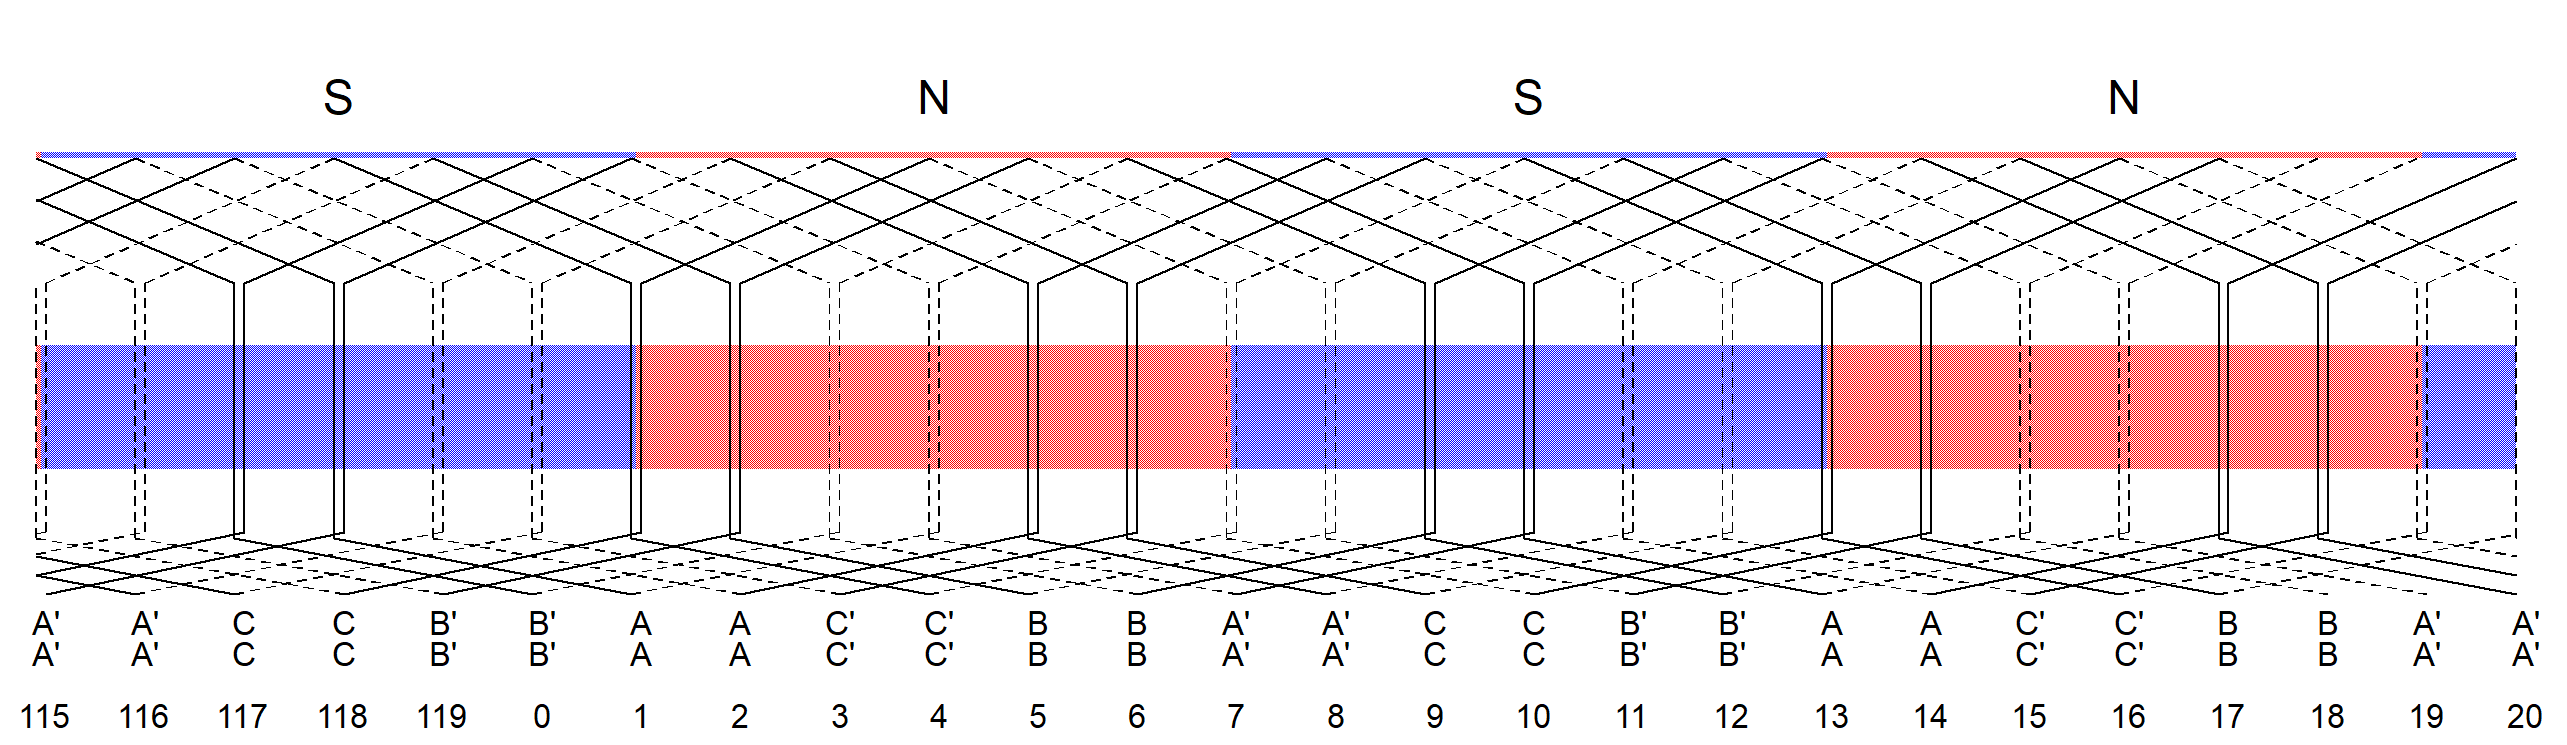
\includegraphics[width=1.0\textwidth]{Q1_windingDiagram_1pp.png}
	\end{center}
	\caption{Winding Diagram: 1 pole pair}
	\label{fig:windingDiagram}
\end{figure}

In Figure \ref{fig:windingDiagram}, above, each pole is indicated with one rectangle, coloured either red or blue, labelled as either \textit{N} or \textit{S}. A single \textit{pole-pair} is composed of two adjacent rectangles, one \textit{N} and one \textit{S}. In Figure \ref{fig:windingDiagram}, one \textit{pole-pair} is corresponding to the slots 1 to 13. As can be seen in the figure, every slot has one side of two different coils, indicating that this is a double layer winding. Number of slots per pole per phase is,
\begin{equation}
q=\frac{Q}{2mp}=2
\end{equation}
meaning there are 2 slots (or 4 half-slots) reserved for coils from excited with each phase. In this machine, \textit{coil-span} is set to be 6 slots. Therefore, the 4 half-slots correspond to 2 slots. In Figure \ref{fig:windingDiagram}, for the pole corresponding to slots 1 to 7, the 2 slots reserved for phase A are slot 1 and 2, the first two slots.
Winding diagram for 120-slot/20-pole configuration, with a \textit{coil-span} of 6 slots, constructed by the software \textit{Dolomites} can be seen in Figure \ref{fig:windingDiagram_dolomites}, below. The complete winding diagram is given in Figure \ref{subfig:winding_dolomites} and in Figure \ref{subfig:winding_1pole_dolomites}, the winding diagram corresponding approximately to one \textit{pole-pair} is given. Though the winding diagram presented by the software \textit{Dolomites} does not display how the coils are wounded, the winding diagram in Figure \ref{fig:windingDiagram} is in compliance with the diagram in Figure \ref{fig:windingDiagram_dolomites}, in terms of coil sequence.

\begin{figure}[h!]
    \centering
    \begin{subfigure}[b]{0.6\textwidth}
        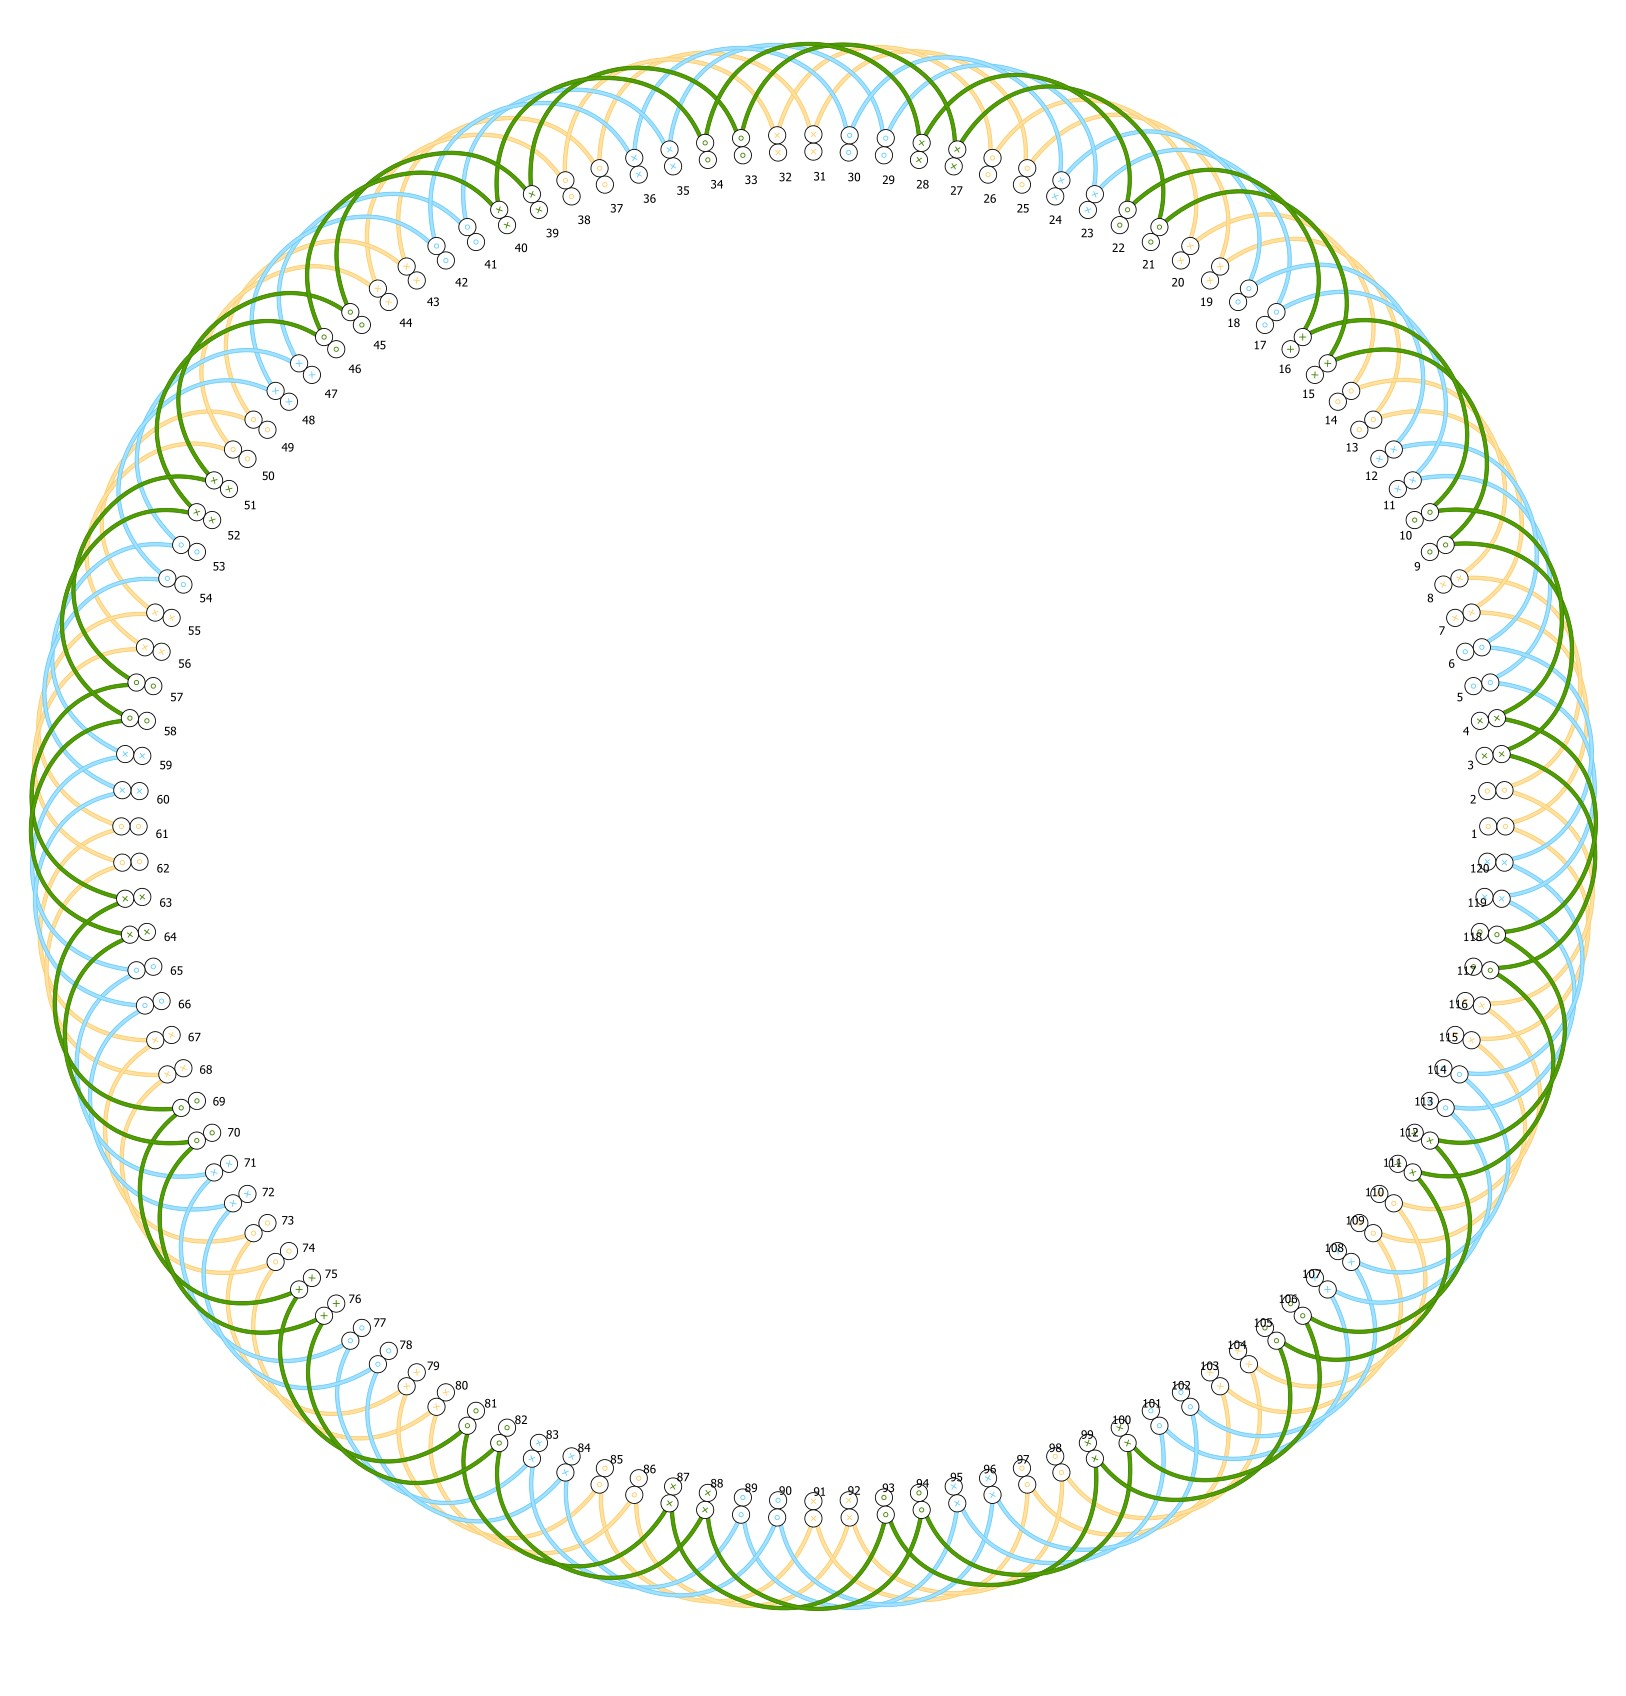
\includegraphics[width=\textwidth]{Q1_windingDiagram_dolomites.jpg}
        \caption{Complete}
        \label{subfig:winding_dolomites}
    \end{subfigure}
    \begin{subfigure}[b]{0.35\textwidth}
        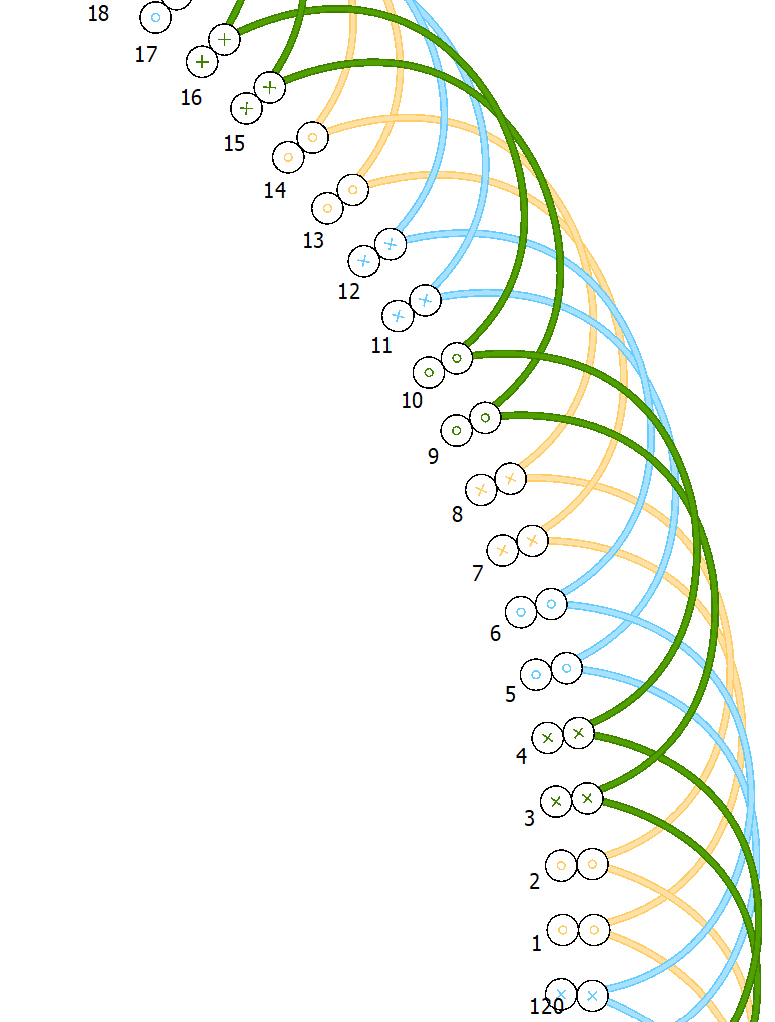
\includegraphics[width=\textwidth]{Q1_windingDiagram_1pp_dolomites.png}
        \vspace{20pt}
        \caption{1 pole-pair}
        \label{subfig:winding_1pole_dolomites}
    \end{subfigure}
    \caption{Winding Diagram}
    \label{fig:windingDiagram_dolomites}
\end{figure}


\subsection{Distribution, Pitch and Winding Factors}

The distribution factor is the ration of the effective induced EMF to arithmetic induced EMF. It can be calculated by

\begin{equation}
K_{dn} = \frac{sin(n\frac{q\sigma}{2})}{qsin(n\frac{\sigma}{2})}
\label{eq:distribution_factor_arithmetic}
\end{equation}

where, \textit{$\sigma$} is the electrical angle between two adjacent coils of the same phase, \textit{q} is the number of coils per phase, and \textit{n} is the harmonic index. Notice that the distribution factor, based on \ref{eq:distribution_factor_arithmetic}, only depends on the electrical angle between two adjacent coils of the same phase and the number of coils per phase. For an integral-slot winding scheme, the choice of phase coils is rather straightforward. However, this choice becomes complicated for a fractional-slot winding scheme, and is detailed in section \ref{subsubsec:phasor_d_2722}.

The pitch factor is the ratio of the effective flux linkage to flux linkage of full-pitched coil. It can be calculated by

\begin{equation}
K_{pn} = \frac{\Psi_s}{\Psi_F}=sin(n\frac{\alpha}{2})
\label{eq:pitch_factor_artihmetic}
\end{equation}

where, \textit{$\Psi_e$} is the effective flux linkage, \textit{$\Psi_F$} is the flux linkage of full-pitched coil, $\alpha$ is the electrical angle of coil pitch, and \textit{n} is the harmonic index. If the coil is full-pitched, then the electrical angle of coil pitch equals to electrical angle of pole pitch (electrical angle pole pitch always equals to 180\degree). In this case, coil links the fundamental and all harmonic flux components. As a result, the coil pitch equals to 1. In case of short pitch or long pitch, the electrical angle of coil pitch differs from electrical angle pole pitch by an electrical angle $A$. This angle, and the corresponding pitch factor is same for both short and long pitch coil.

The winding factor is the ratio of the effective winding turns to actual winding turns. It can be calculated by

\begin{equation}
K_{wn} = K_{dn}K_{pn}
\label{eq:pitch_factor}
\end{equation}


Distribution, pitch, and the winding factors for 120-slot/20-pole machine is given in Figure \ref{fig:Q1_factors_12020}, for n=1,3,...,21. Additionally, the fundamental and the 3\textsuperscript{rd} and 5\textsuperscript{th} harmonics for each factor are given in Table \ref{tab:Q1_factors_12020}. These factors values are identical to those presented by the software \textit{Dolomites} and the website \textit{Emetor}.

\begin{table}[h!]
\centering
	\begin{tabular}{|c| c c c|} 
		\hline
		n & 1 & 2 & 2 \\ [0.5ex] 
		\hline
		Distribution Factor & 0.9659 & 0.7071 & 0.2588 \\ 
		\hline
		Pitch Factor & 1 & 1 & 1 \\
		\hline
		Winding Factor & 0.9659 & 0.7071 & 0.2588 \\
		\hline
	\end{tabular}
	\caption{Distribution, Pitch and Winding Factor for $\frac{N_s}{2p}=120/20$}
	\label{tab:Q1_factors_12020}
\end{table}



\begin{figure}[h!]
    \centering
    \begin{subfigure}[b]{1.00\textwidth}
        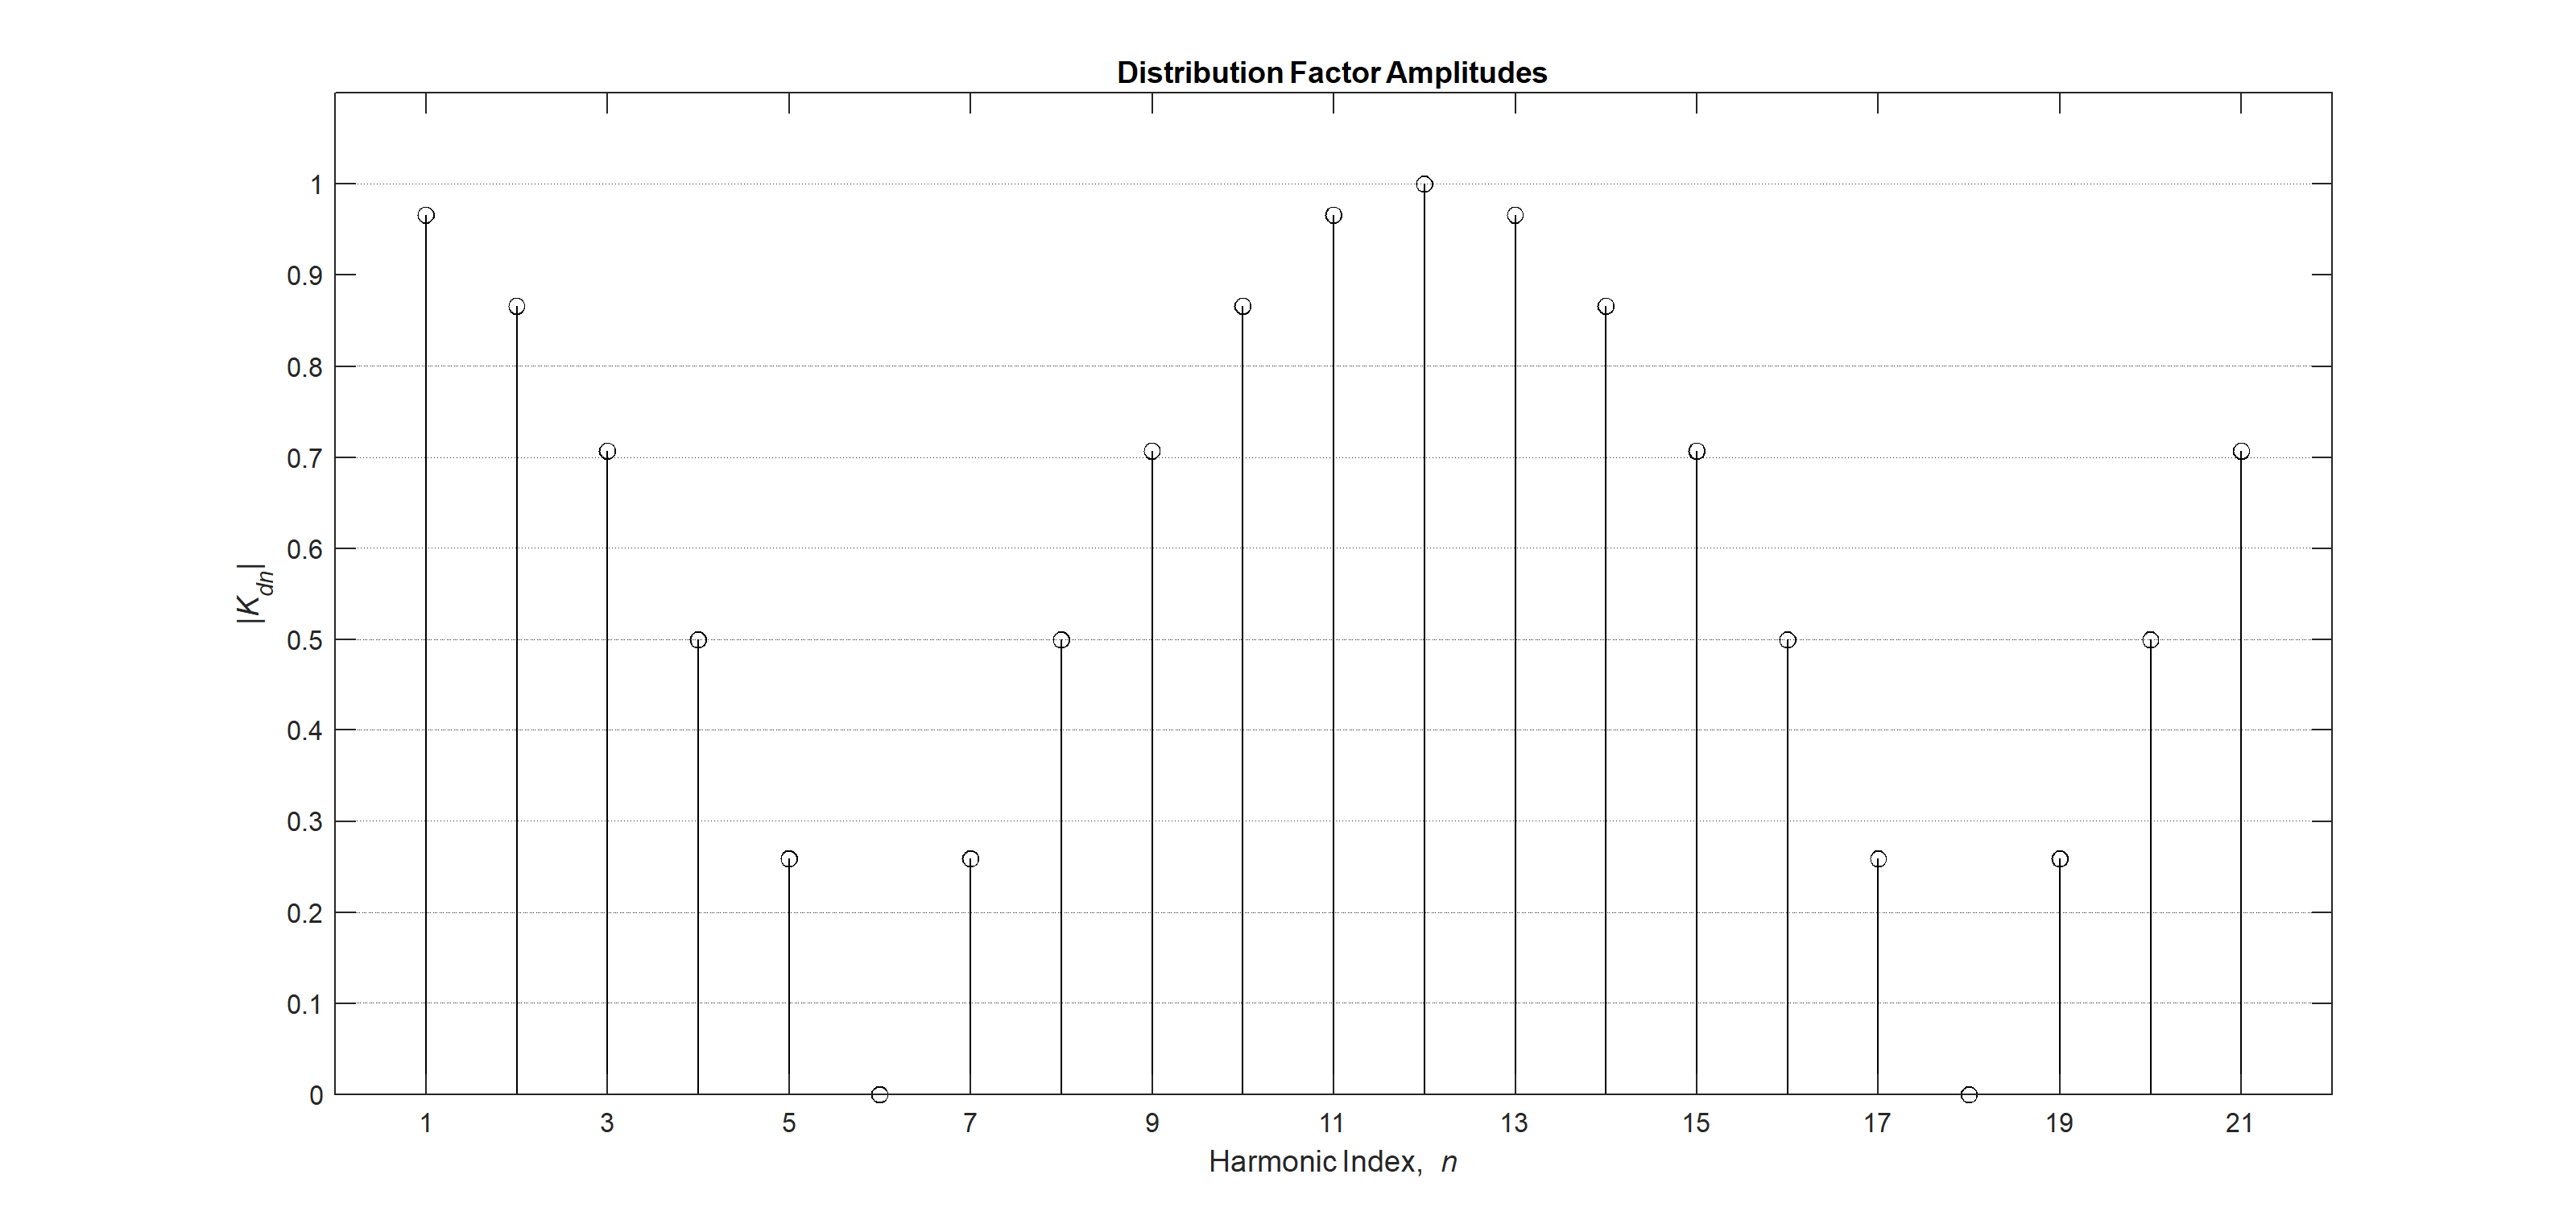
\includegraphics[width=\textwidth]{Q1_distributionFactor.png}
        \caption{}
        \label{subfig:Q1_dist_factor}
    \end{subfigure}
    \begin{subfigure}[b]{1.00\textwidth}
        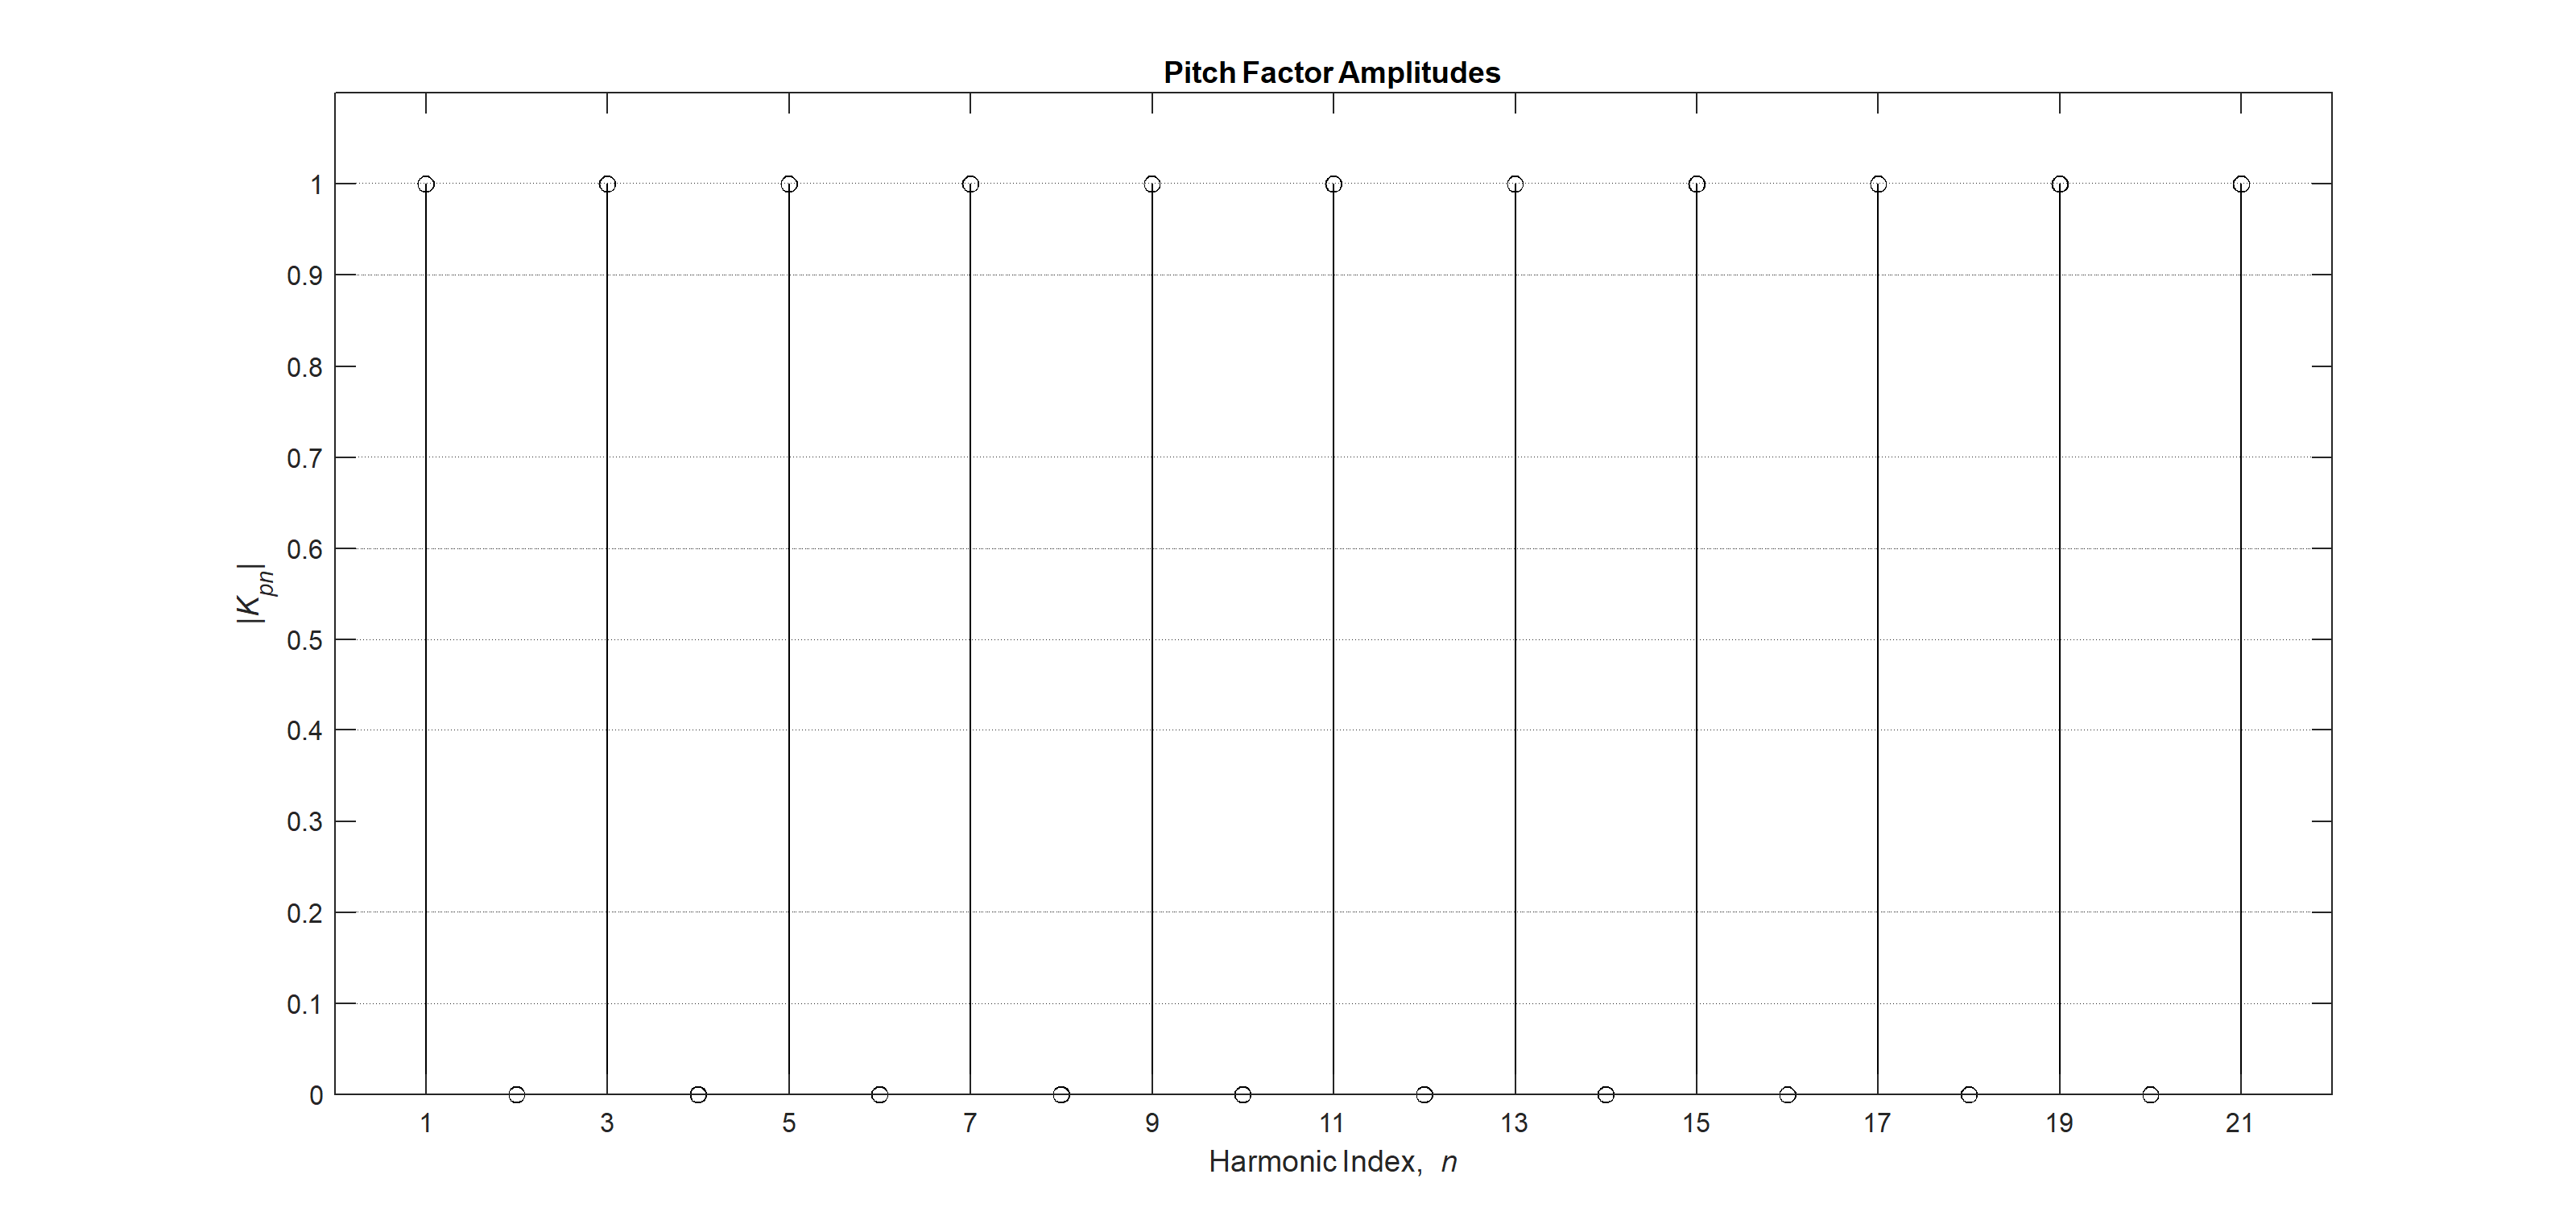
\includegraphics[width=\textwidth]{Q1_pitchFactor.png}
        \caption{}
        \label{subfig:Q1_pitch_factor}
    \end{subfigure}
    \begin{subfigure}[b]{1.00\textwidth}
        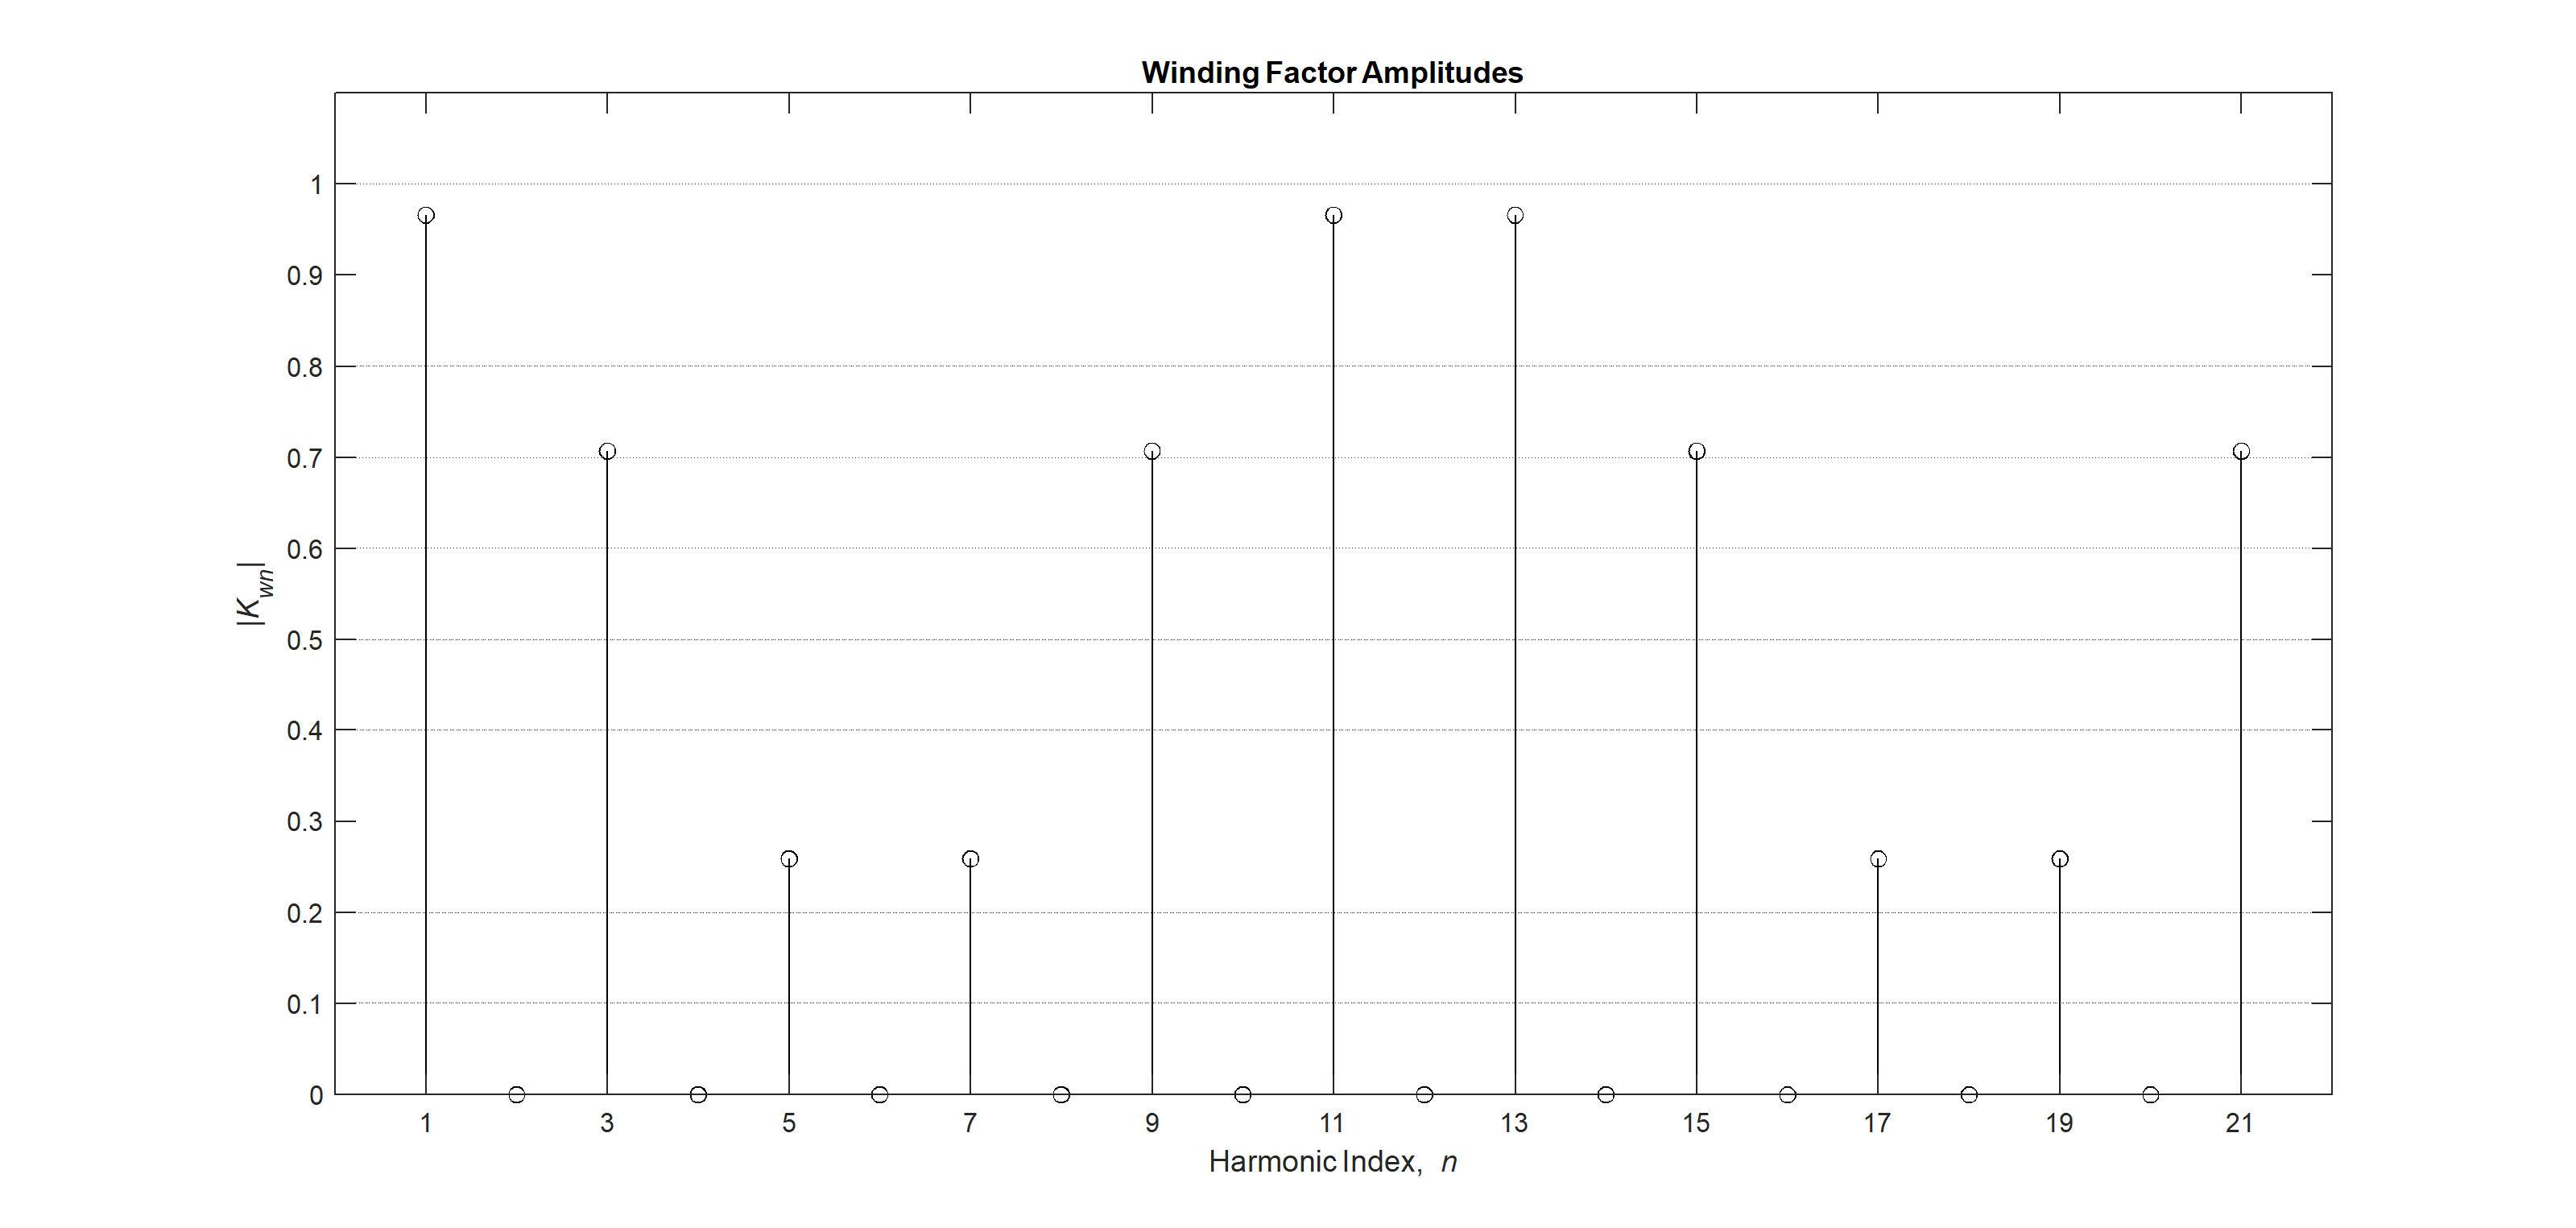
\includegraphics[width=\textwidth]{Q1_windingFactor.png}
        \caption{}
        \label{subfig:Q1_wind_factor}
    \end{subfigure}
    \caption{Distribution, Pitch and Winding Factor for $\frac{N_s}{2p}=120/20$}
    \label{fig:Q1_factors_12020}
\end{figure}


It is expected to have a unit pitch factor, while the \textit{coil-span} of the machine is selected to be 6 slots, which equals to the pole span, which is $\frac{Q}{2p}=6$  slots.

The fundamental component of distribution factor is high, an important aspect for an integral slot winding, as it is directly proportinal to sunisoidality of the MMF, however, the 3\textsuperscript{rd} and 5\textsuperscript{th} harmonic components alters the MMF waveform away from a perfect sunisoidal form; thus, not desired. Here, for the $\frac{N_s}{2p}=120/20$ configuration, the fundamental component of the winding factor is $K_{w1} =0.9659$, high and well above acceptable levels. However, 3\textsuperscript{rd} and 5\textsuperscript{th} harmonic components of the winding factor are $K_{w3} =0.7071$ and $K_{w5} =0.2588$, which are high, deforming the waveform away from its sinusiodality. A scaled MMF waveform according to the fundamental, 3\textsuperscript{rd} and 5\textsuperscript{th} harmonic component values given in Table \ref{tab:Q1_factors_12020} can be seen in Figure \ref{fig:MMFWaveform}.

\begin{figure}[h]
	\begin{center}
		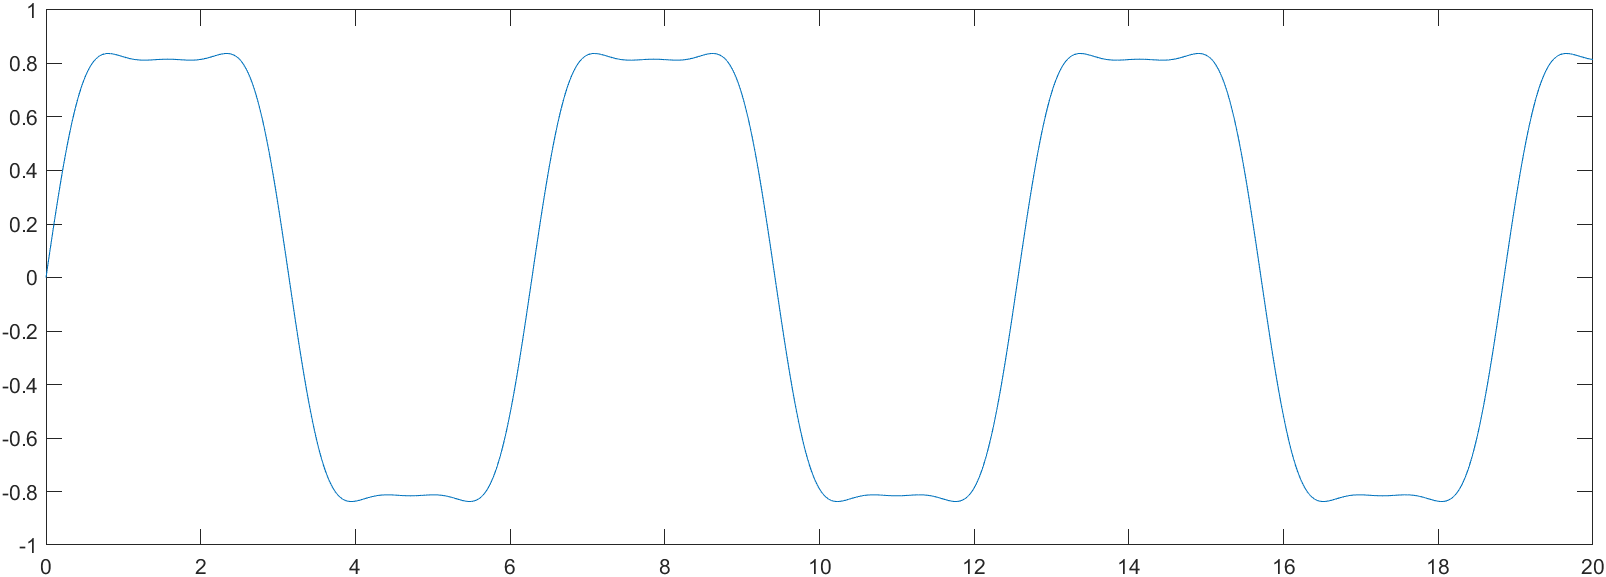
\includegraphics[width=0.9\textwidth]{Q1_MMFWaveform.png}
	\end{center}
	\caption{Waveform with $\frac{N_s}{2p}=120/20$ winding factors (1\textsuperscript{st}, 3\textsuperscript{rd} and 5\textsuperscript{th})}
	\label{fig:MMFWaveform}
\end{figure}


\section{Fractional-Slot Winding Design}

Fractional-slot refers to machine topologies in which the number of slots per pole per phase is an fractional number.

\begin{equation}
q=\frac{Q}{2pm}
\end{equation}

\begin{equation}
q\notin N
\end{equation}


\subsection{27-slot/22-pole EM}

\label{subsec:fractional-slot}

The first fractional-slot electric machine analysed in this project is a 27-slot 22-pole machine. An electric machine with such slot/pole ($\frac{N_s}{2p}$) configuration can only be constructed as double-layer (all teeth wound). In a double-layer design, the \textit{coil-span} can vary. This project adopts a design where each coil spans 1 slots. This choice depends on the theory that the coil pitch needs to be closer to the pole pitch to obtain a higher pitch factor. Here, \textit{pole-pitch} is $\frac{2\pi}{2p}$ and \textit{slot-pitch} is $\frac{2\pi}{sQ}$, where \textit{s} is the \textit{coil-span}. Therefore, to obtain the highest pitch factor, \textit{coil-span} is chosen to be 1.

\subsubsection{Phase Angle of Induced Voltage in each Slot}

The phase shift between each coil can be calculated as

\begin{equation}
phase shift=\frac{2\pi}{Q/2p}
\end{equation}

Phase angles of the induced voltages in each slot are presented in Table \ref{tab:ph_ang_2722}, below.

\begin{table}[h!]
\centering
	\begin{tabular}{||c|| c c c c c c||} 
		\hline\hline
		Slot Number & 1 & 2 & 3 & 4 & 5 & 6\\ [0.5ex] 
		\hline
		Phase Angle (\degree) & 0 & 146.67 & 293.33 & 80 & 226.67 & 13.33\\ 
		\hline\hline
		& 7 & 8 & 9 & 10 & 11 & 12\\
		\hline
		& 160 & 306.67 & 93.33 & 240 & 26.67 & 173.33\\
		\hline\hline
		& 13 & 14 & 15 & 16 & 17 & 18\\
		\hline
		& 320 & 106.67 & 253.33 & 40 & 186.67 & 333.33\\
	 	\hline\hline
		& 19 & 20 & 21 & 22 & 23 & 24\\
		\hline
		& 120 & 266.67 & 53.33 & 200 & 346.67 & 133.33\\
		\hline\hline
		& 25 & 26 & 27\\
		\hline
		& 280 & 66.67 & 213.33\\
		\hline\hline
	\end{tabular}
	\caption{Phase angle of the induced voltage for $\frac{N_s}{2p}=27/22$}
	\label{tab:ph_ang_2722}
\end{table}


\subsubsection{Phasor Diagram}
\label{subsubsec:phasor_d_2722}

One method to represent the main EMF harmonic which are being induced at the coil side is referref as star of slots. The star of slots method uses phasors to represent the EMFs and this representation comprises each of the slots \cite{bianchi}.

The star of slots representation method is used to represent the machine with $\frac{N_s}{2p}=27/22$. The representation with mechanical angles can be seen in Figure \ref{subfig:sos_2722_mech}, with electrical angles can be seen in Figure \ref{subfig:sos_2722_elec}. The star of slots representation with electrical angles implements the phasors according to the phase angle values presented in Table \ref{tab:ph_ang_2722}


\begin{figure}[h!]
    \centering
    \begin{subfigure}[b]{0.45\textwidth}
        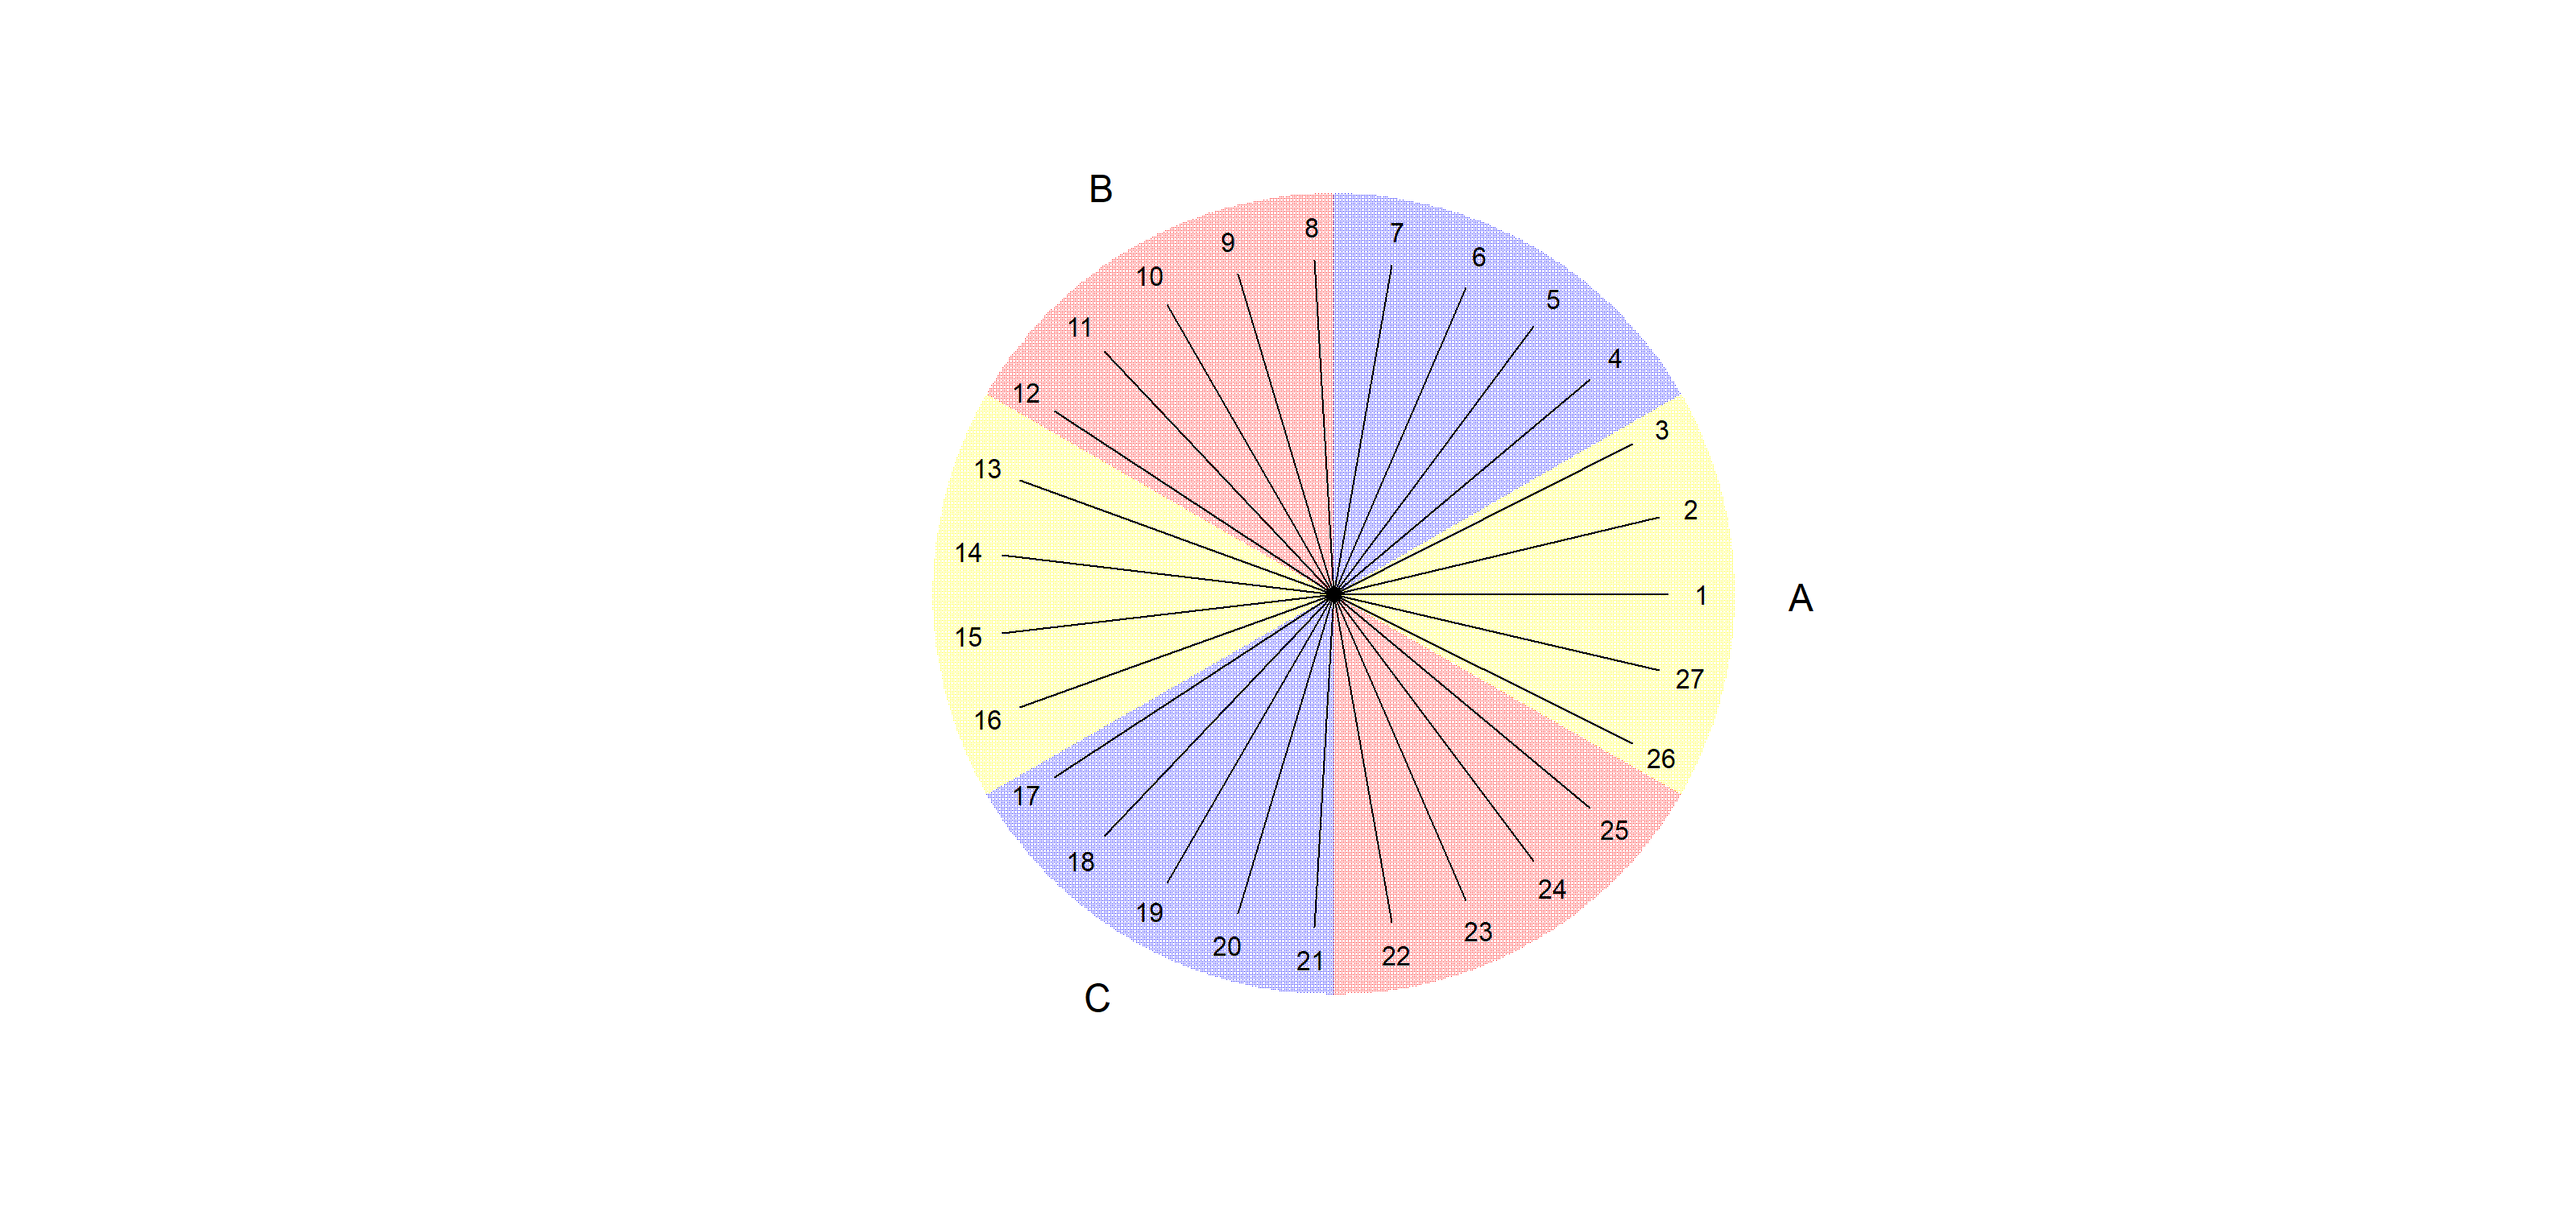
\includegraphics[width=\textwidth]{Q2_2722_starofSlots_mechanical.png}
        \caption{mechanical}
        \label{subfig:sos_2722_mech}
    \end{subfigure}
    ~ %add desired spacing between images, e. g. ~, \quad, \qquad, \hfill etc. 
      %(or a blank line to force the subfigure onto a new line)
    \begin{subfigure}[b]{0.45\textwidth}
        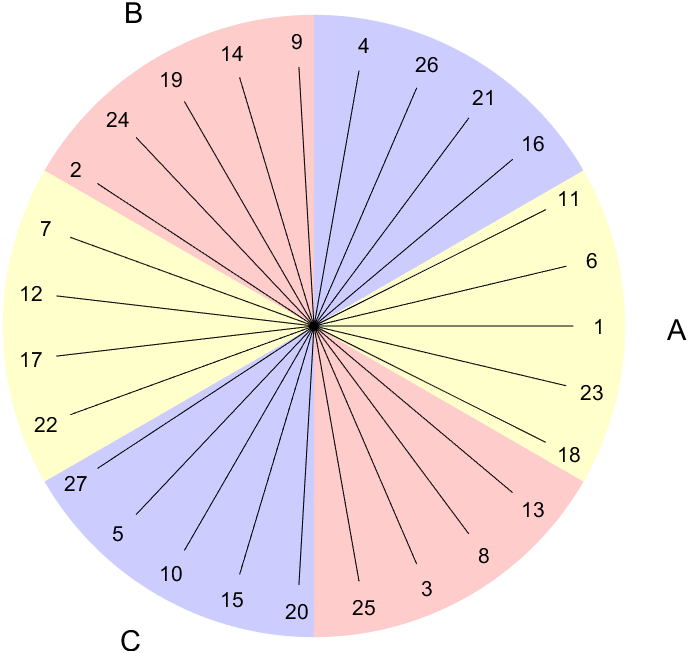
\includegraphics[width=\textwidth]{Q2_2722_starofSlots_electrical.png}
        \caption{electrical}
        \label{subfig:sos_2722_elec}
    \end{subfigure}
    \caption{Star of Slots for $\frac{N_s}{2p}=27/22$}
    \label{fig:sos_2722}
\end{figure}


Once the star of slots representation with electrical angles is completed, the coils for each phase are selected. This selection is done according to which phasors lie on which $2\pi/6$ area. As can be seen in Figure \ref{fig:sos_2722_wSectors}, The slots corresponding to the phasors which lie on the yellow, or phase A area, are chosen to be wound with phase A coils.



\begin{figure}[h!]
    \centering
	\begin{center}
		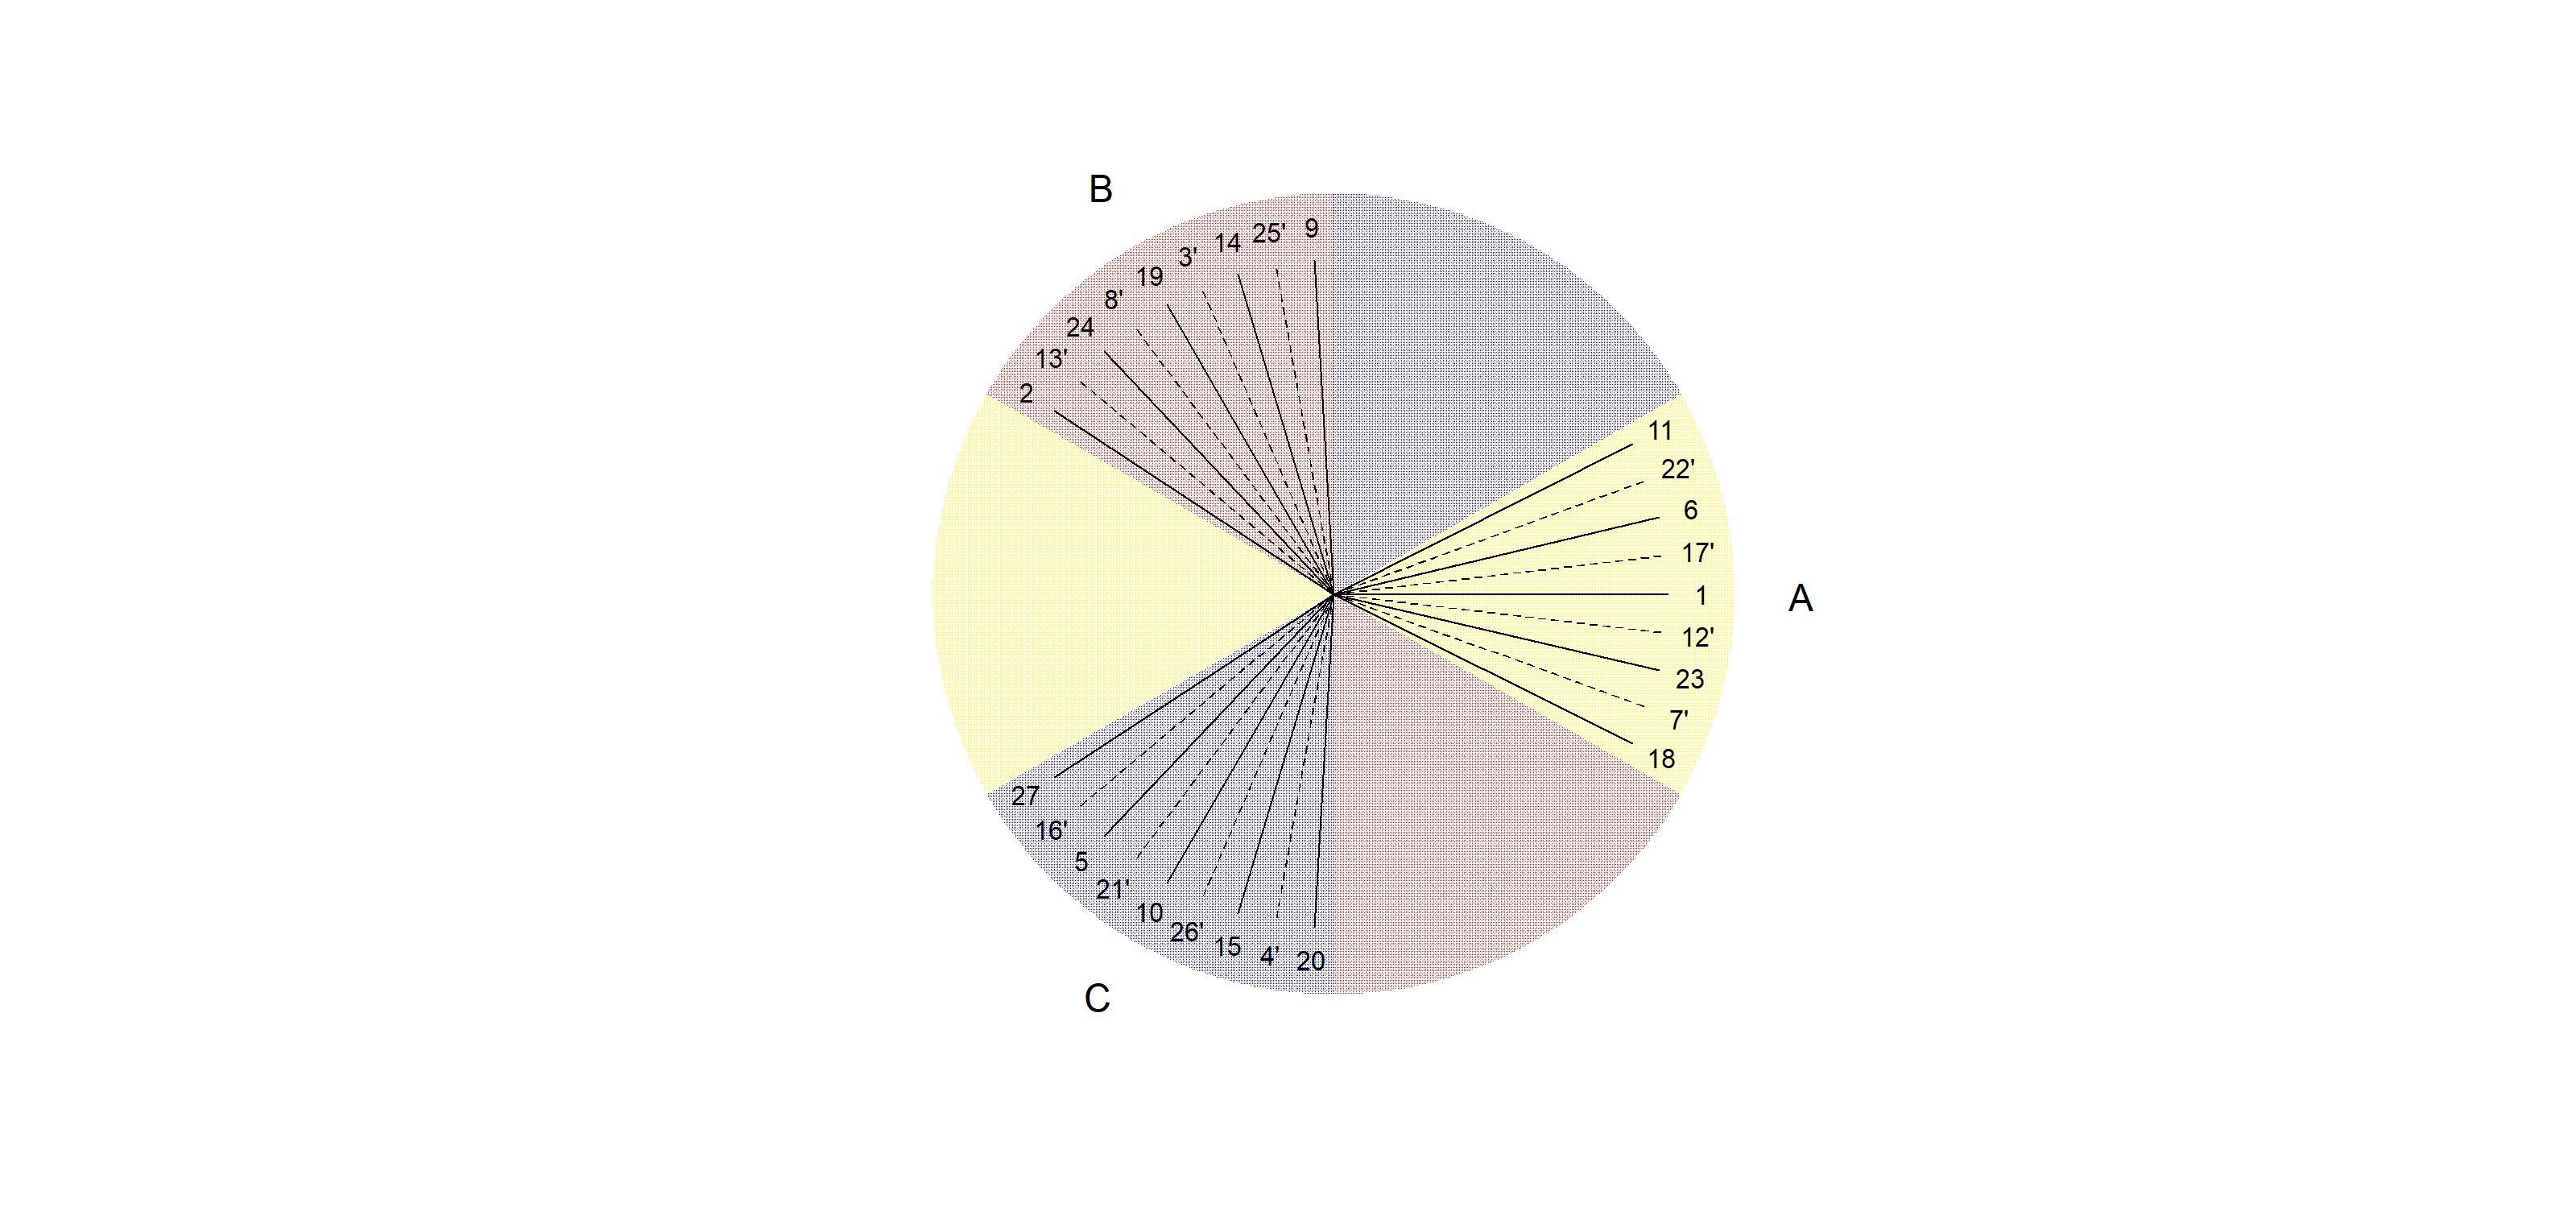
\includegraphics[width=0.6\textwidth]{Q2_2722_phasorDiagram_wSectors.png}
	\end{center}
	\caption{Star of Slots for $\frac{N_s}{2p}=27/22$ (according to the coil direction)}
	\label{fig:sos_2722_wSectors}
\end{figure}

Finally, the phasor can be represented with a phasor diagram, where phasors from each phase are displayed in an additive manner. The phasor diagram for phase A for the $\frac{N_s}{2p}=27/22$ topology can be seen in Figure \ref{fig:phasor_d_2722}.


\begin{figure}[h!]
    \centering
	\begin{center}
		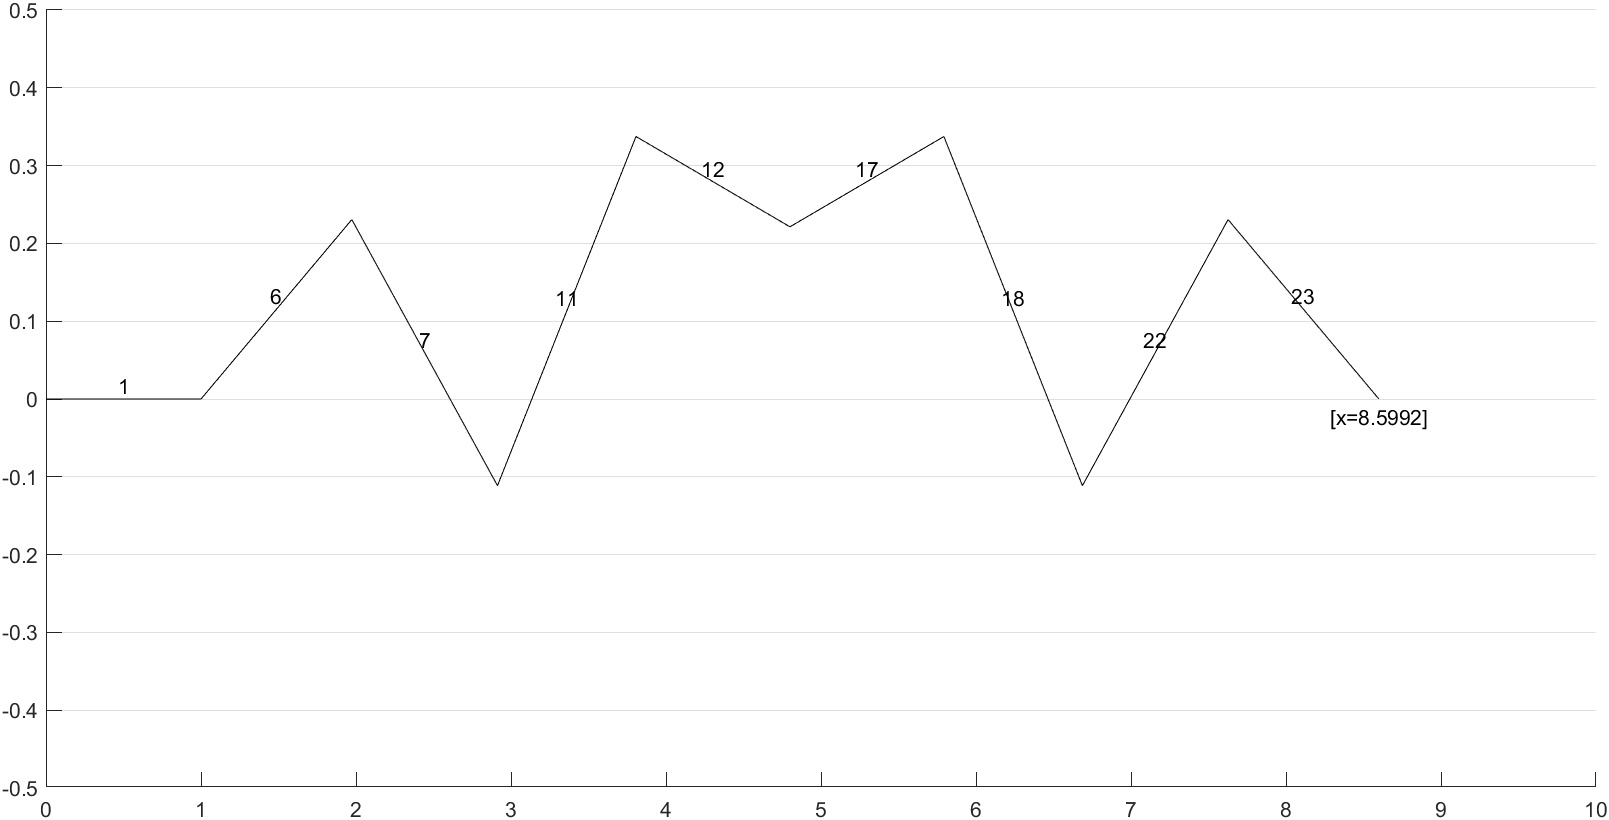
\includegraphics[width=1.0\textwidth]{Q2_2722_phasorDiagram_1ph.png}
	\end{center}
	\caption{Phasor Diagram for $\frac{N_s}{2p}=27/22$ (phase A)}
	\label{fig:phasor_d_2722}
\end{figure}

It is important to note here that the distribution factor can be deduced from the phasor diagram. Notice that there are 9 phasors in phase A, which corresponds to arithmetic induced EMF, scaled by peak induced EMF per coil. These phasors add up to the point [x,y]=[8.5992], which corresponds to effective induced EMF. Thus, the distribution factor is

\begin{equation}
K_{dn} = \frac{effective induced EMF}{arithmetic induced EMF}=\frac{8.5992}{9}=0.9555
\label{eq:distribution_factor_phasor}
\end{equation}



\subsubsection{Distribution, Pitch and Winding Factors}



Distribution, pitch, and the winding factors for 27-slot/22-pole machine is given in Figure \ref{fig:Q2_factors_2722}, for n=1,3,...,21. Additionally, the fundamental and the 3\textsuperscript{rd} and 5\textsuperscript{th} harmonics for each factor are given in Table \ref{tab:Q2_factors_2722}. These factors values are identical to those presented by the software \textit{Dolomites} and the website \textit{Emetor}.


\begin{table}[h!]
\centering
	\begin{tabular}{|c| c c c|} 
		\hline
		n & 1 & 2 & 2 \\ [0.5ex] 
		\hline
		Distribution Factor & 0.9555 & 0.6399 & 0.1937 \\ 
		\hline
		Pitch Factor & 0.9580 & 0.6428 & 0.1161 \\
		\hline
		Winding Factor & 0.9153 & 0.4113 & 0.0225 \\
		\hline
	\end{tabular}
	\caption{Distribution, Pitch and Winding Factor for $\frac{N_s}{2p}=27/22$}
	\label{tab:Q2_factors_2722}
\end{table}


\begin{figure}[h!]
    \centering
    \begin{subfigure}[b]{1.00\textwidth}
        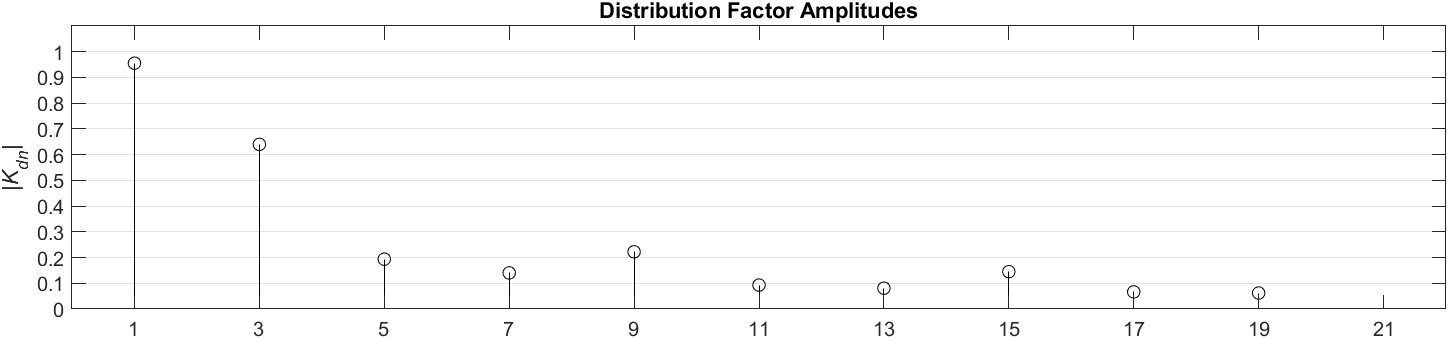
\includegraphics[width=\textwidth]{Q2_2722_distributionFactor.png}
        \caption{}
        \label{subfig:Q2_dist_factor_2722}
    \end{subfigure}
    \begin{subfigure}[b]{1.00\textwidth}
        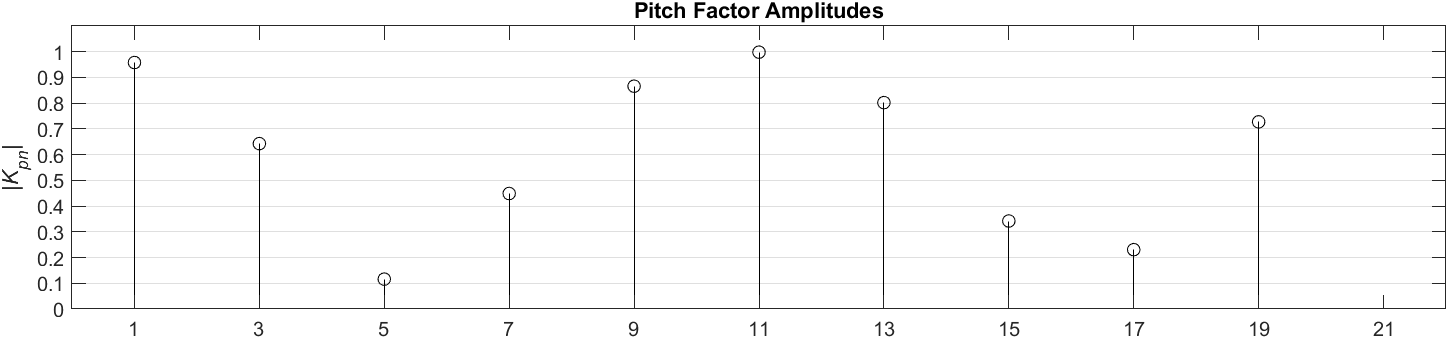
\includegraphics[width=\textwidth]{Q2_2722_pitchFactor.png}
        \caption{}
        \label{subfig:Q2_pitch_factor_2722}
    \end{subfigure}
    \begin{subfigure}[b]{1.00\textwidth}
        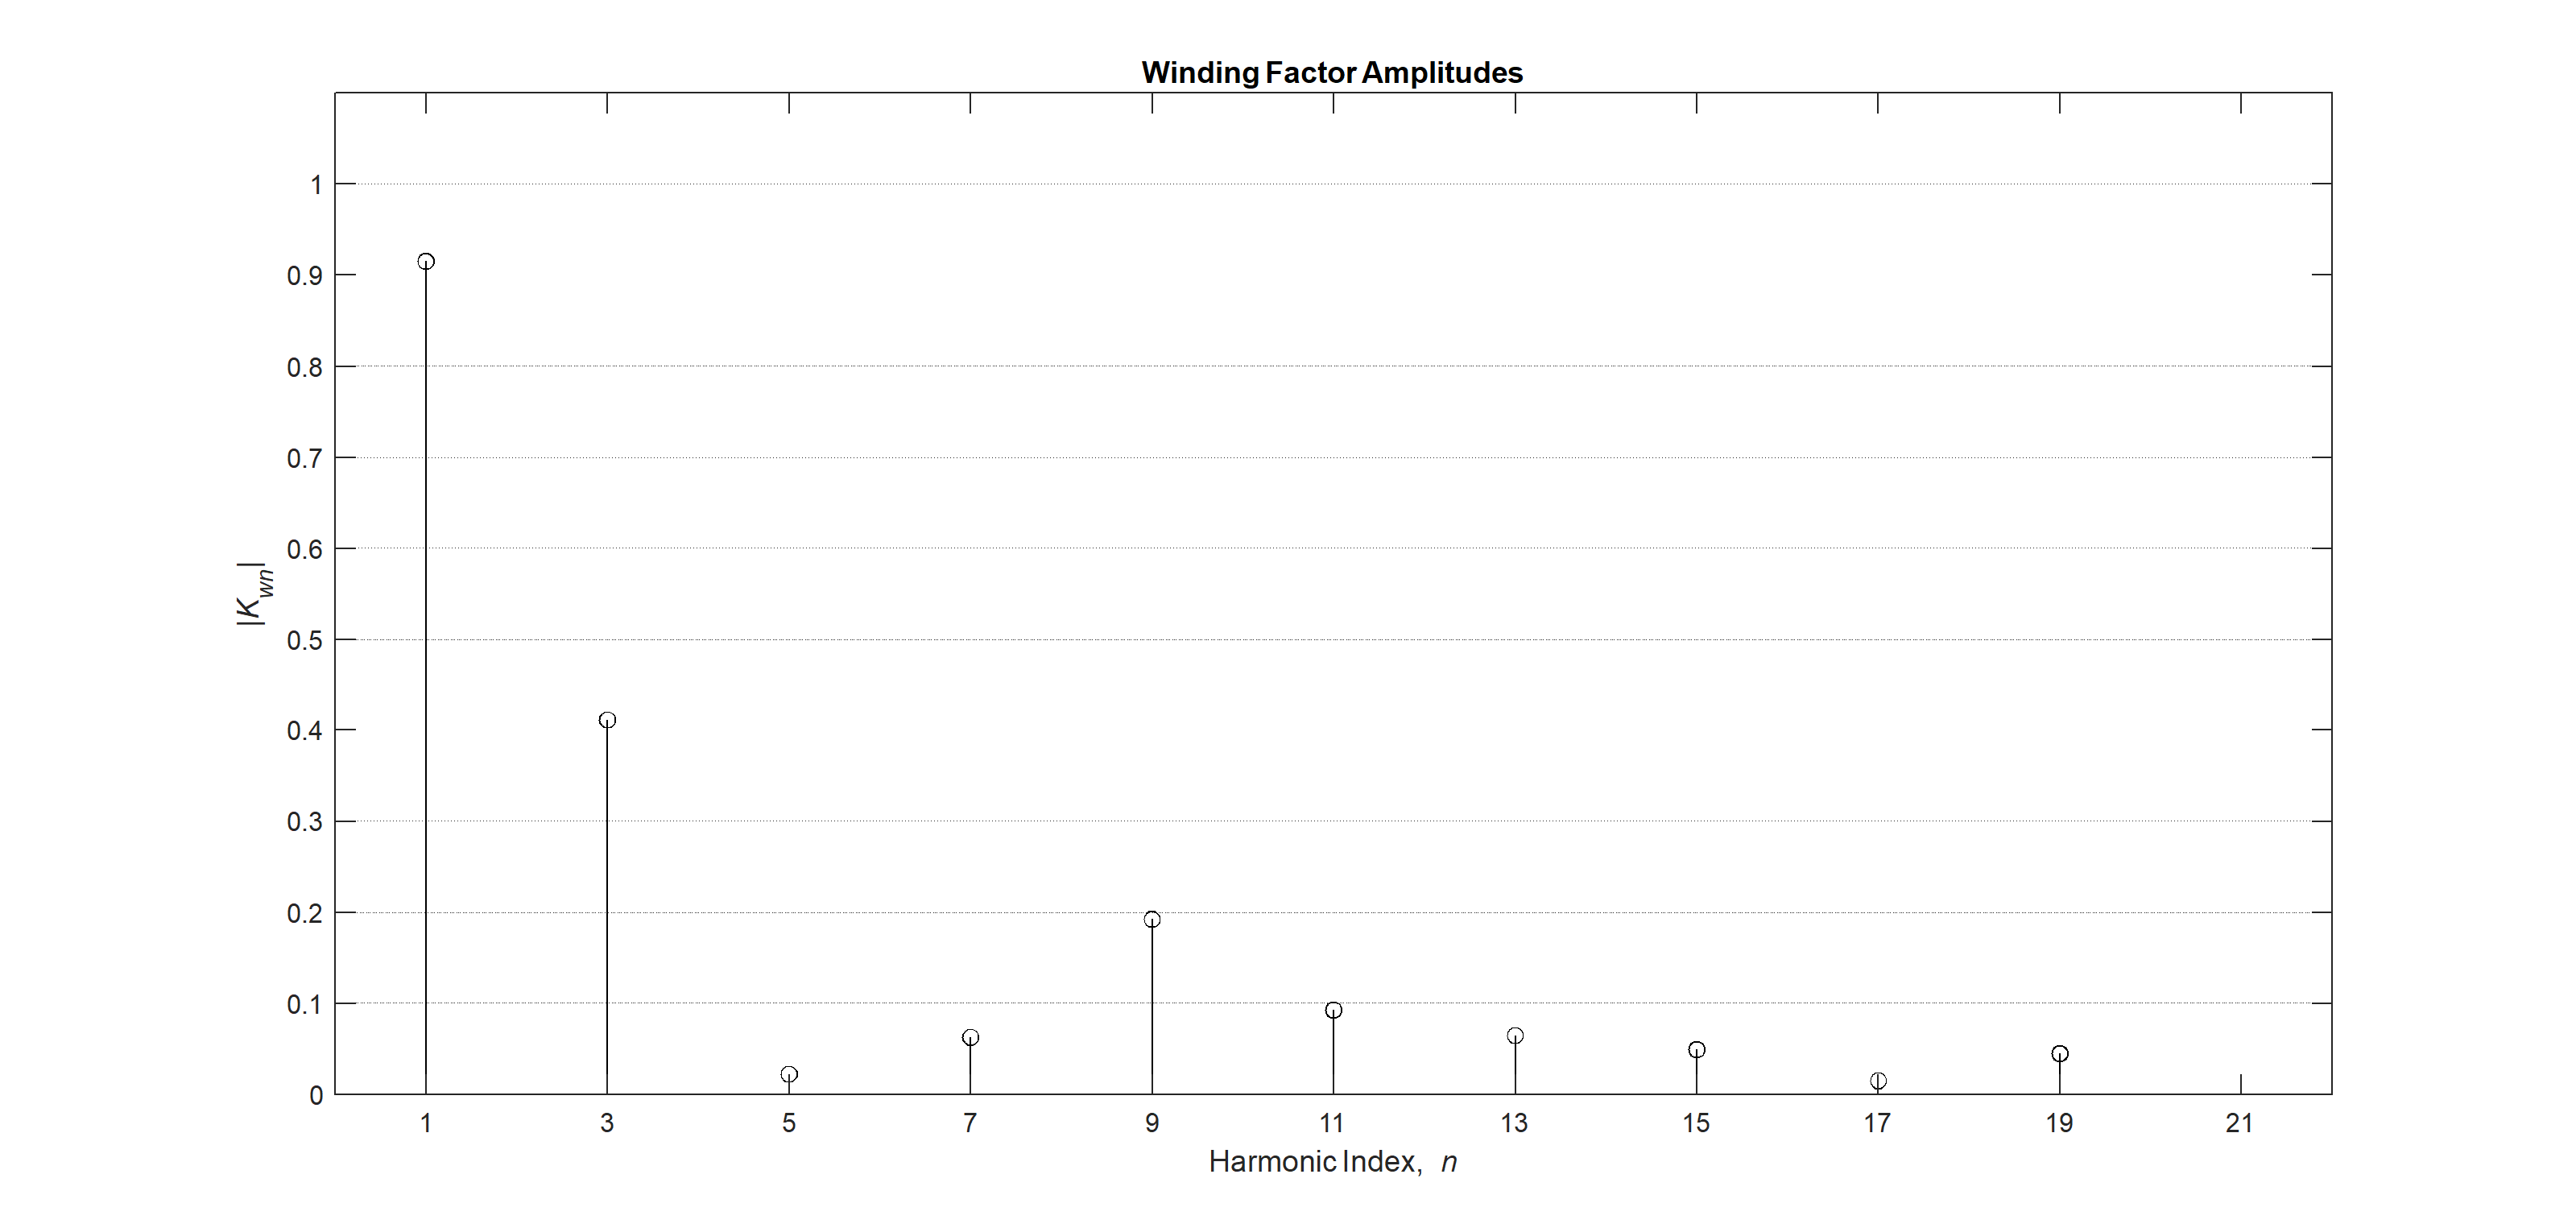
\includegraphics[width=\textwidth]{Q2_2722_windingFactor.png}
        \caption{}
        \label{subfig:Q2_wind_factor_2722}
    \end{subfigure}
    \caption{Distribution, Pitch and Winding Factor for $\frac{N_s}{2p}=27/22$}
    \label{fig:Q2_factors_2722}
\end{figure}

As can be seen in Figure \ref{tab:Q2_factors_2722}, the fundamental distribution factor calculated analytically with the Equation \ref{eq:distribution_factor_arithmetic} gives the same results with that calculated by the phasor diagram in \ref{subsubsec:phasor_d_2722}.





\subsection{24-slot/22-pole EM}

The second fractional-slot electric machine analysed in this project is a 24-slot 22-pole machine. An electric machine with such slot/pole ($\frac{N_s}{2p}$) configuration can only be constructed either as single-layer (alternate teeth wound) or double-layer (all teeth wound). In a double-layer design, the \textit{coil-span} can vary. This project adopts a double-layer design, where each coil spans 1 slots. The choice of \textit{coil-span} is done with the same grounds explained in Subsection \ref{subsec:fractional-slot}.

\subsubsection{Phase Angle of Induced Voltage in each Slot}

Phase angles of the induced voltages in each slot are presented in Table \ref{tab:ph_ang_2422}, below.

\begin{table}[ht!]
\centering
	\begin{tabular}{|c| c c c c c c|} 
		\hline\hline
		Slot Number & 1 & 2 & 3 & 4 & 5 & 6\\ [0.5ex] 
		\hline
		Phase Angle (\degree) & 0 & 165 & 330 &135 & 300 & 105\\ 
		\hline\hline
		 & 7 & 8 & 9 & 10 & 11 & 12\\
		\hline
		 & 270 & 75 & 240 & 45 & 210 & 15\\
		\hline\hline
		 & 13 & 14 & 15 & 16 & 17 & 18\\
		 \hline
		  & 180 & 345 & 150 & 315 & 120 & 285\\
		  \hline\hline
		  & 19 & 20 & 21 & 22 & 23 & 24\\
		  \hline
		  & 90 & 255 & 60 & 225 & 30 &195\\
		  \hline\hline
	\end{tabular}
	\caption{Phase angle of the induced voltage}
	\label{tab:ph_ang_2422}
\end{table}


\subsubsection{Phasor Diagram}
\label{subsubsec:phasor_d_2422}

The star of slots method and the phasor diagram is completed for the machine with $\frac{N_s}{2p}=24/22$. The results can be seen in Figure \ref{fig:sos_2422}, \ref{fig:sos_2422_wSectors} and \ref{fig:phasor_d_2422} displayed below.

\begin{figure}[h]
    \centering
    \begin{subfigure}[b]{0.45\textwidth}
        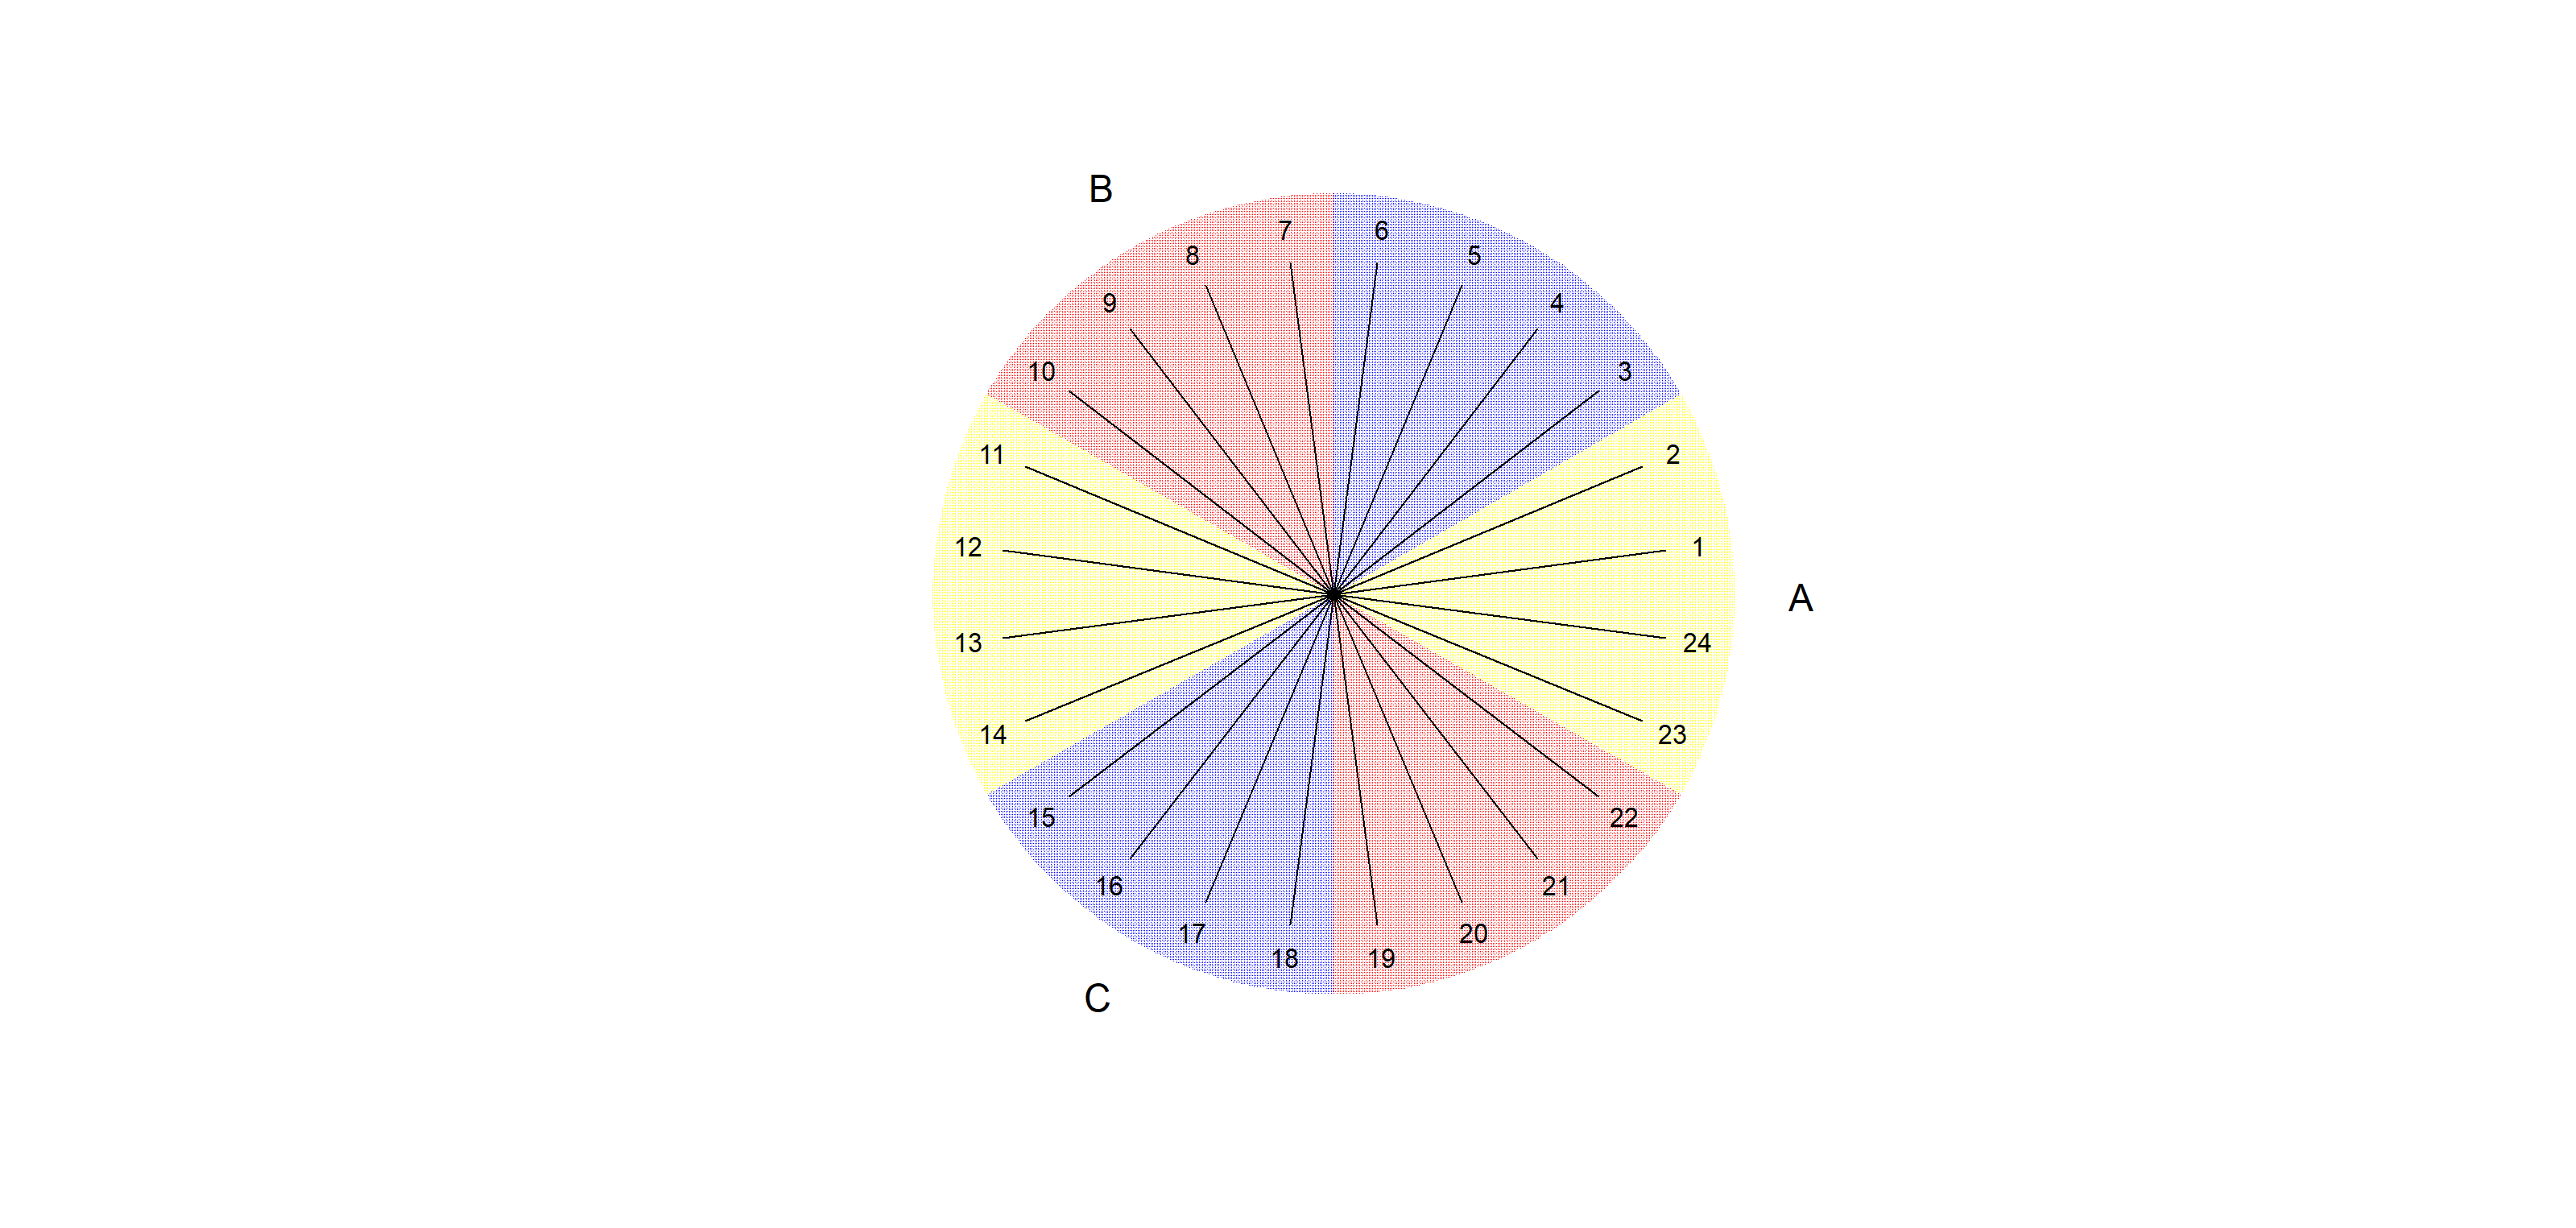
\includegraphics[width=\textwidth]{Q2_2422_starofSlots_mechanical.png}
        \caption{mechanical}
        \label{subfig:sos_2422_mech}
    \end{subfigure}
    \begin{subfigure}[b]{0.45\textwidth}
        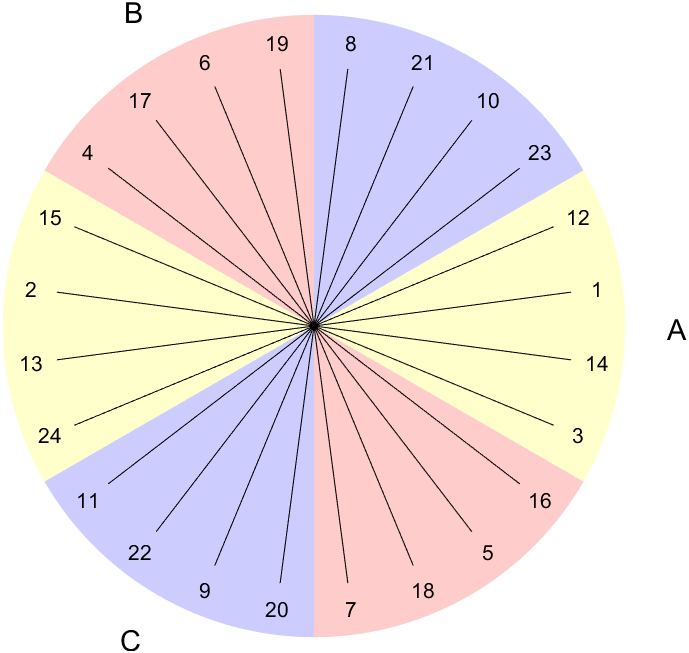
\includegraphics[width=\textwidth]{Q2_2422_starofSlots_electrical.png}
        \caption{electrical}
        \label{subfig:sos_2422_elec}
    \end{subfigure}
    \caption{Star of Slots for $\frac{N_s}{2p}=24/22$}
    \label{fig:sos_2422}
\end{figure}


\begin{figure}[h!]
	\begin{center}
		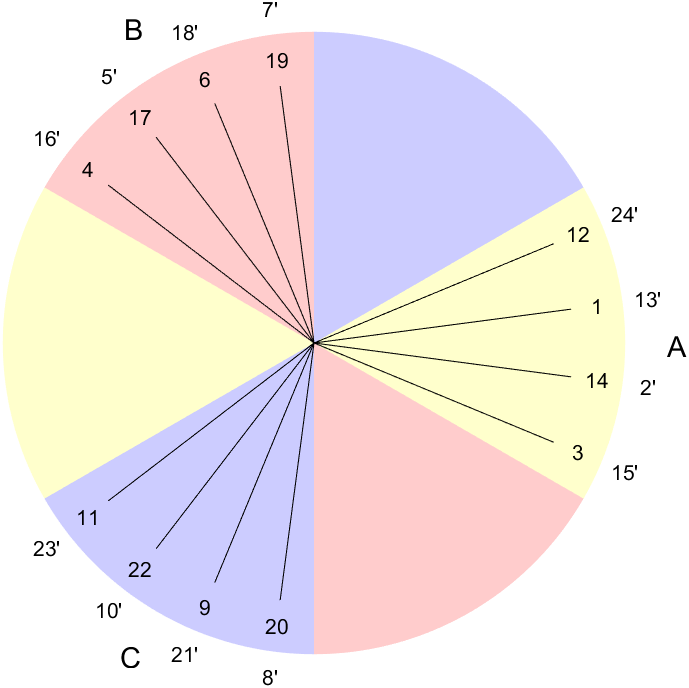
\includegraphics[width=0.6\textwidth]{Q2_2422_phasorDiagram_wSectors.png}
	\end{center}
	\caption{Star of Slots for $\frac{N_s}{2p}=24/22$ (according to the winding direction)}
	\label{fig:sos_2422_wSectors}
\end{figure}

\begin{figure}[h!]
	\begin{center}
		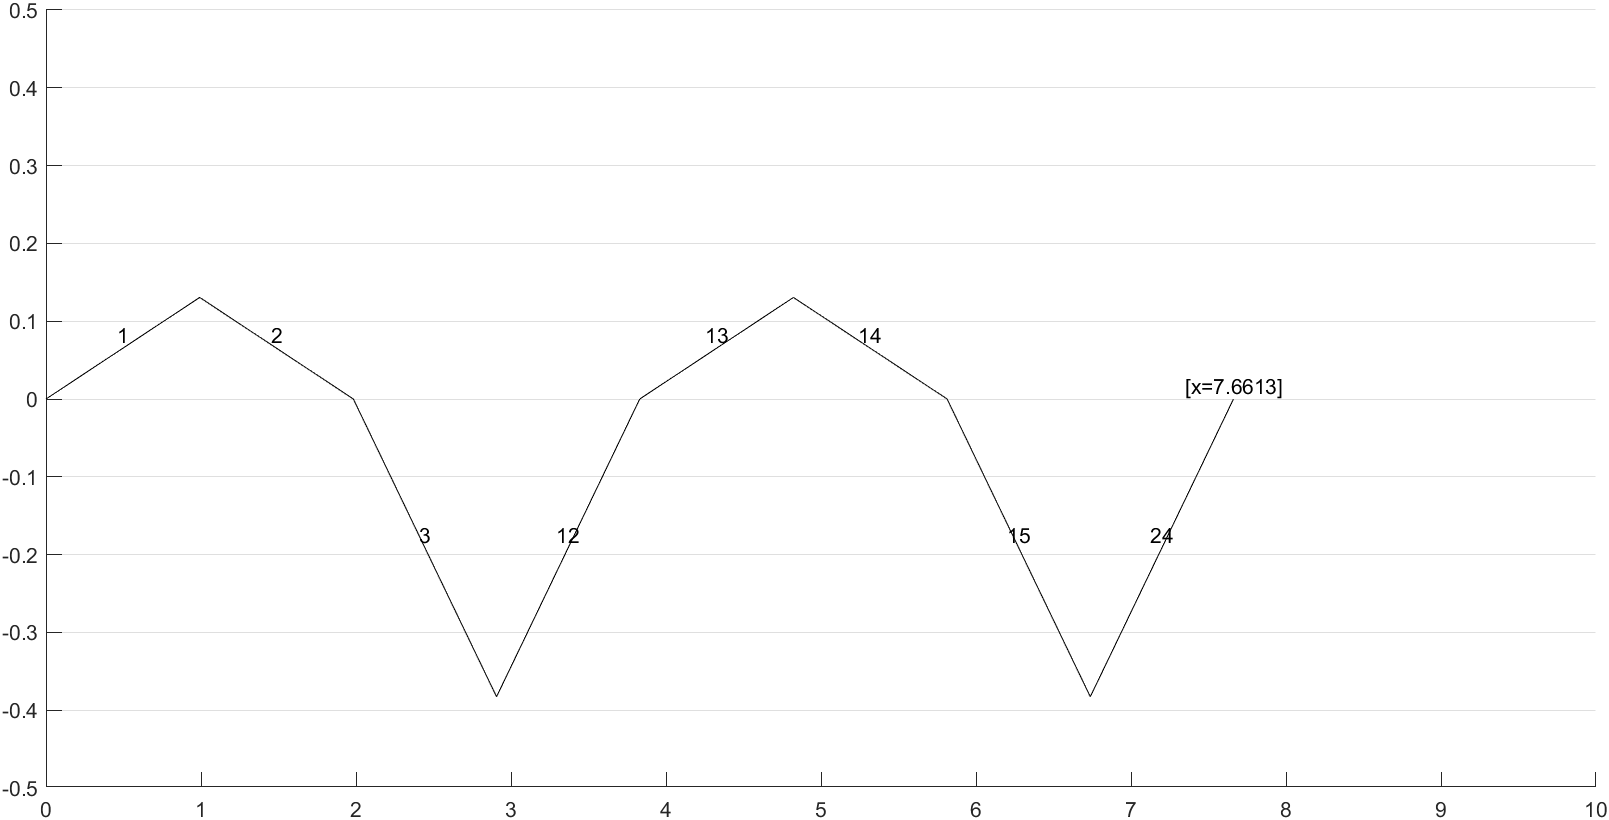
\includegraphics[width=1.0\textwidth]{Q2_2422_phasorDiagram_1ph.png}
	\end{center}
	\caption{Phasor Diagram for $\frac{N_s}{2p}=27/22$ (phase A)}
	\label{fig:phasor_d_2422}
\end{figure}

Again, the distribution factor can be deduced from the phasor diagram here. Notice that there are 8 phasors in phase A, which corresponds to arithmetic induced EMF, scaled by peak induced EMF per coil. These phasors add up to the point [x,y]=[7.6613], which corresponds to effective induced EMF. Thus, the distribution factor is

\begin{equation}
K_{dn} = \frac{effective induced EMF}{arithmetic induced EMF}=\frac{7.6613}{8}=0.9577
\label{eq:distribution_factor_phasor}
\end{equation}


\subsubsection{Distribution, Pitch and Winding Factors}

Distribution, pitch, and the winding factors for 24-slot/22-pole machine is given in Figure \ref{fig:Q2_factors_2422}, for n=1,3,...,21. Additionally, the fundamental and the 3\textsuperscript{rd} and 5\textsuperscript{th} harmonics for each factor are given in Table \ref{tab:Q2_factors_2422}. These factors values are identical to those presented by the software \textit{Dolomites} and the website \textit{Emetor}.

\begin{table}[h!]
\centering
	\begin{tabular}{|c| c c c|} 
		\hline
		n & 1 & 2 & 2 \\ [0.5ex] 
		\hline
		Distribution Factor & 0.9577 & 0.6533 & 0.2053 \\ 
		\hline
		Pitch Factor & 0.9914 & 0.9239 & 0.7934 \\
		\hline
		Winding Factor & 0.9495 & 0.6036 & 0.1629 \\
		\hline
	\end{tabular}
	\caption{Distribution, Pitch and Winding Factor for $\frac{N_s}{2p}=24/22$}
	\label{tab:Q2_factors_2422}
\end{table}


\begin{figure}[h!]
    \centering
    \begin{subfigure}[b]{1.00\textwidth}
        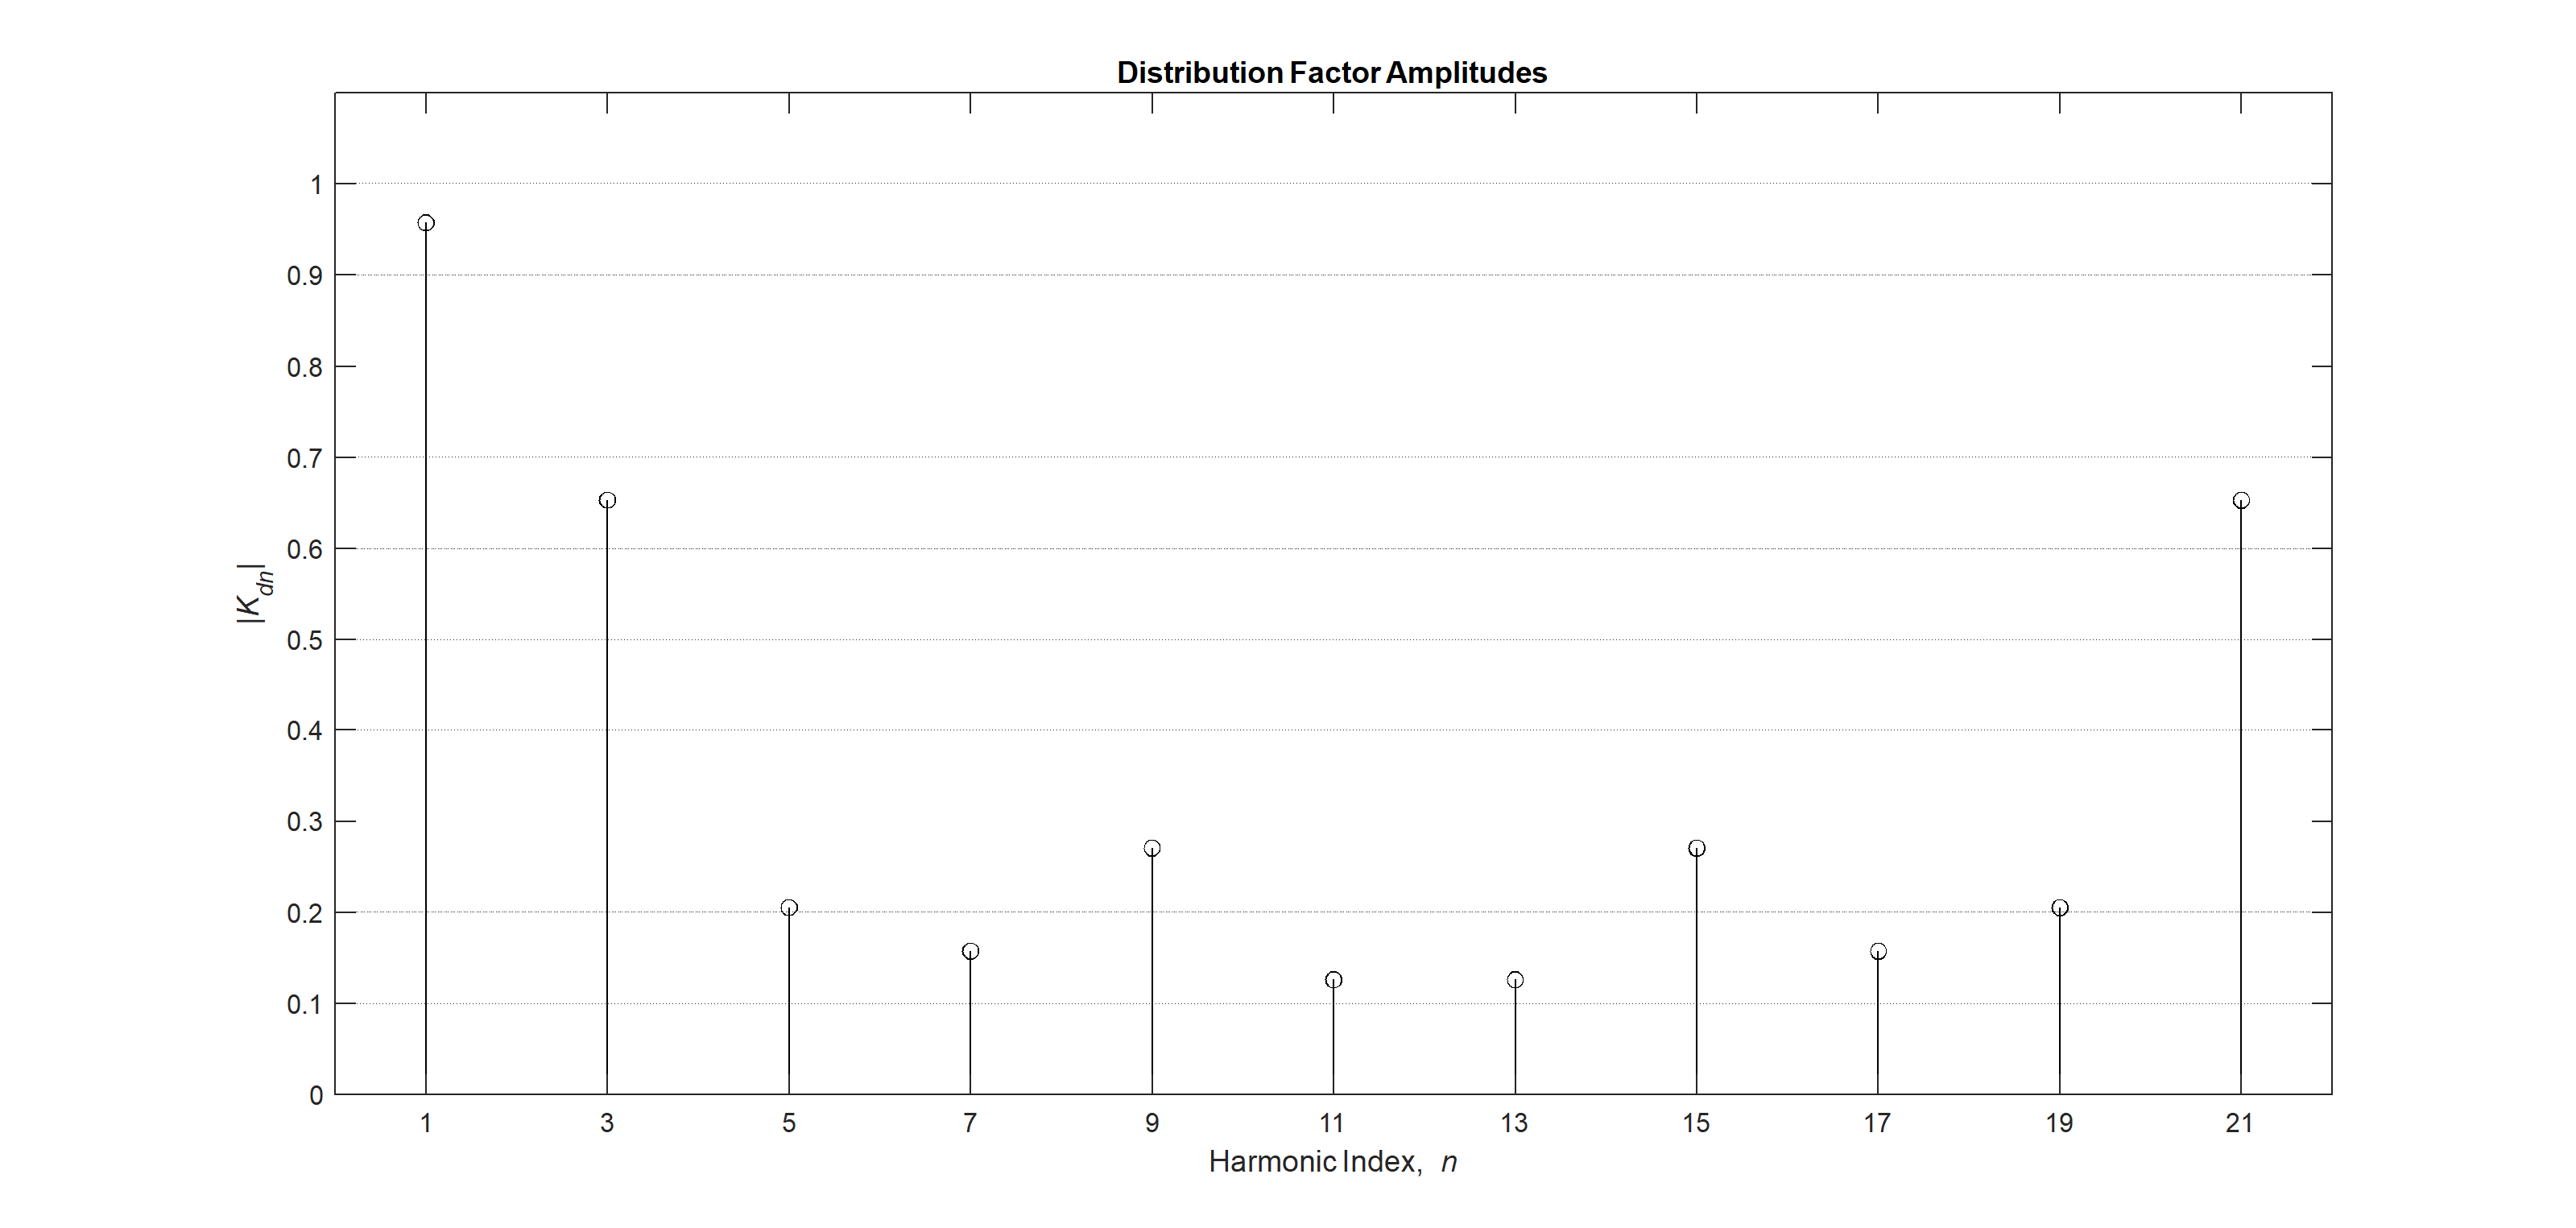
\includegraphics[width=\textwidth]{Q2_2422_distributionFactor.png}
        \caption{}
        \label{subfig:Q2_dist_factor_2422}
    \end{subfigure}
    \begin{subfigure}[b]{1.00\textwidth}
        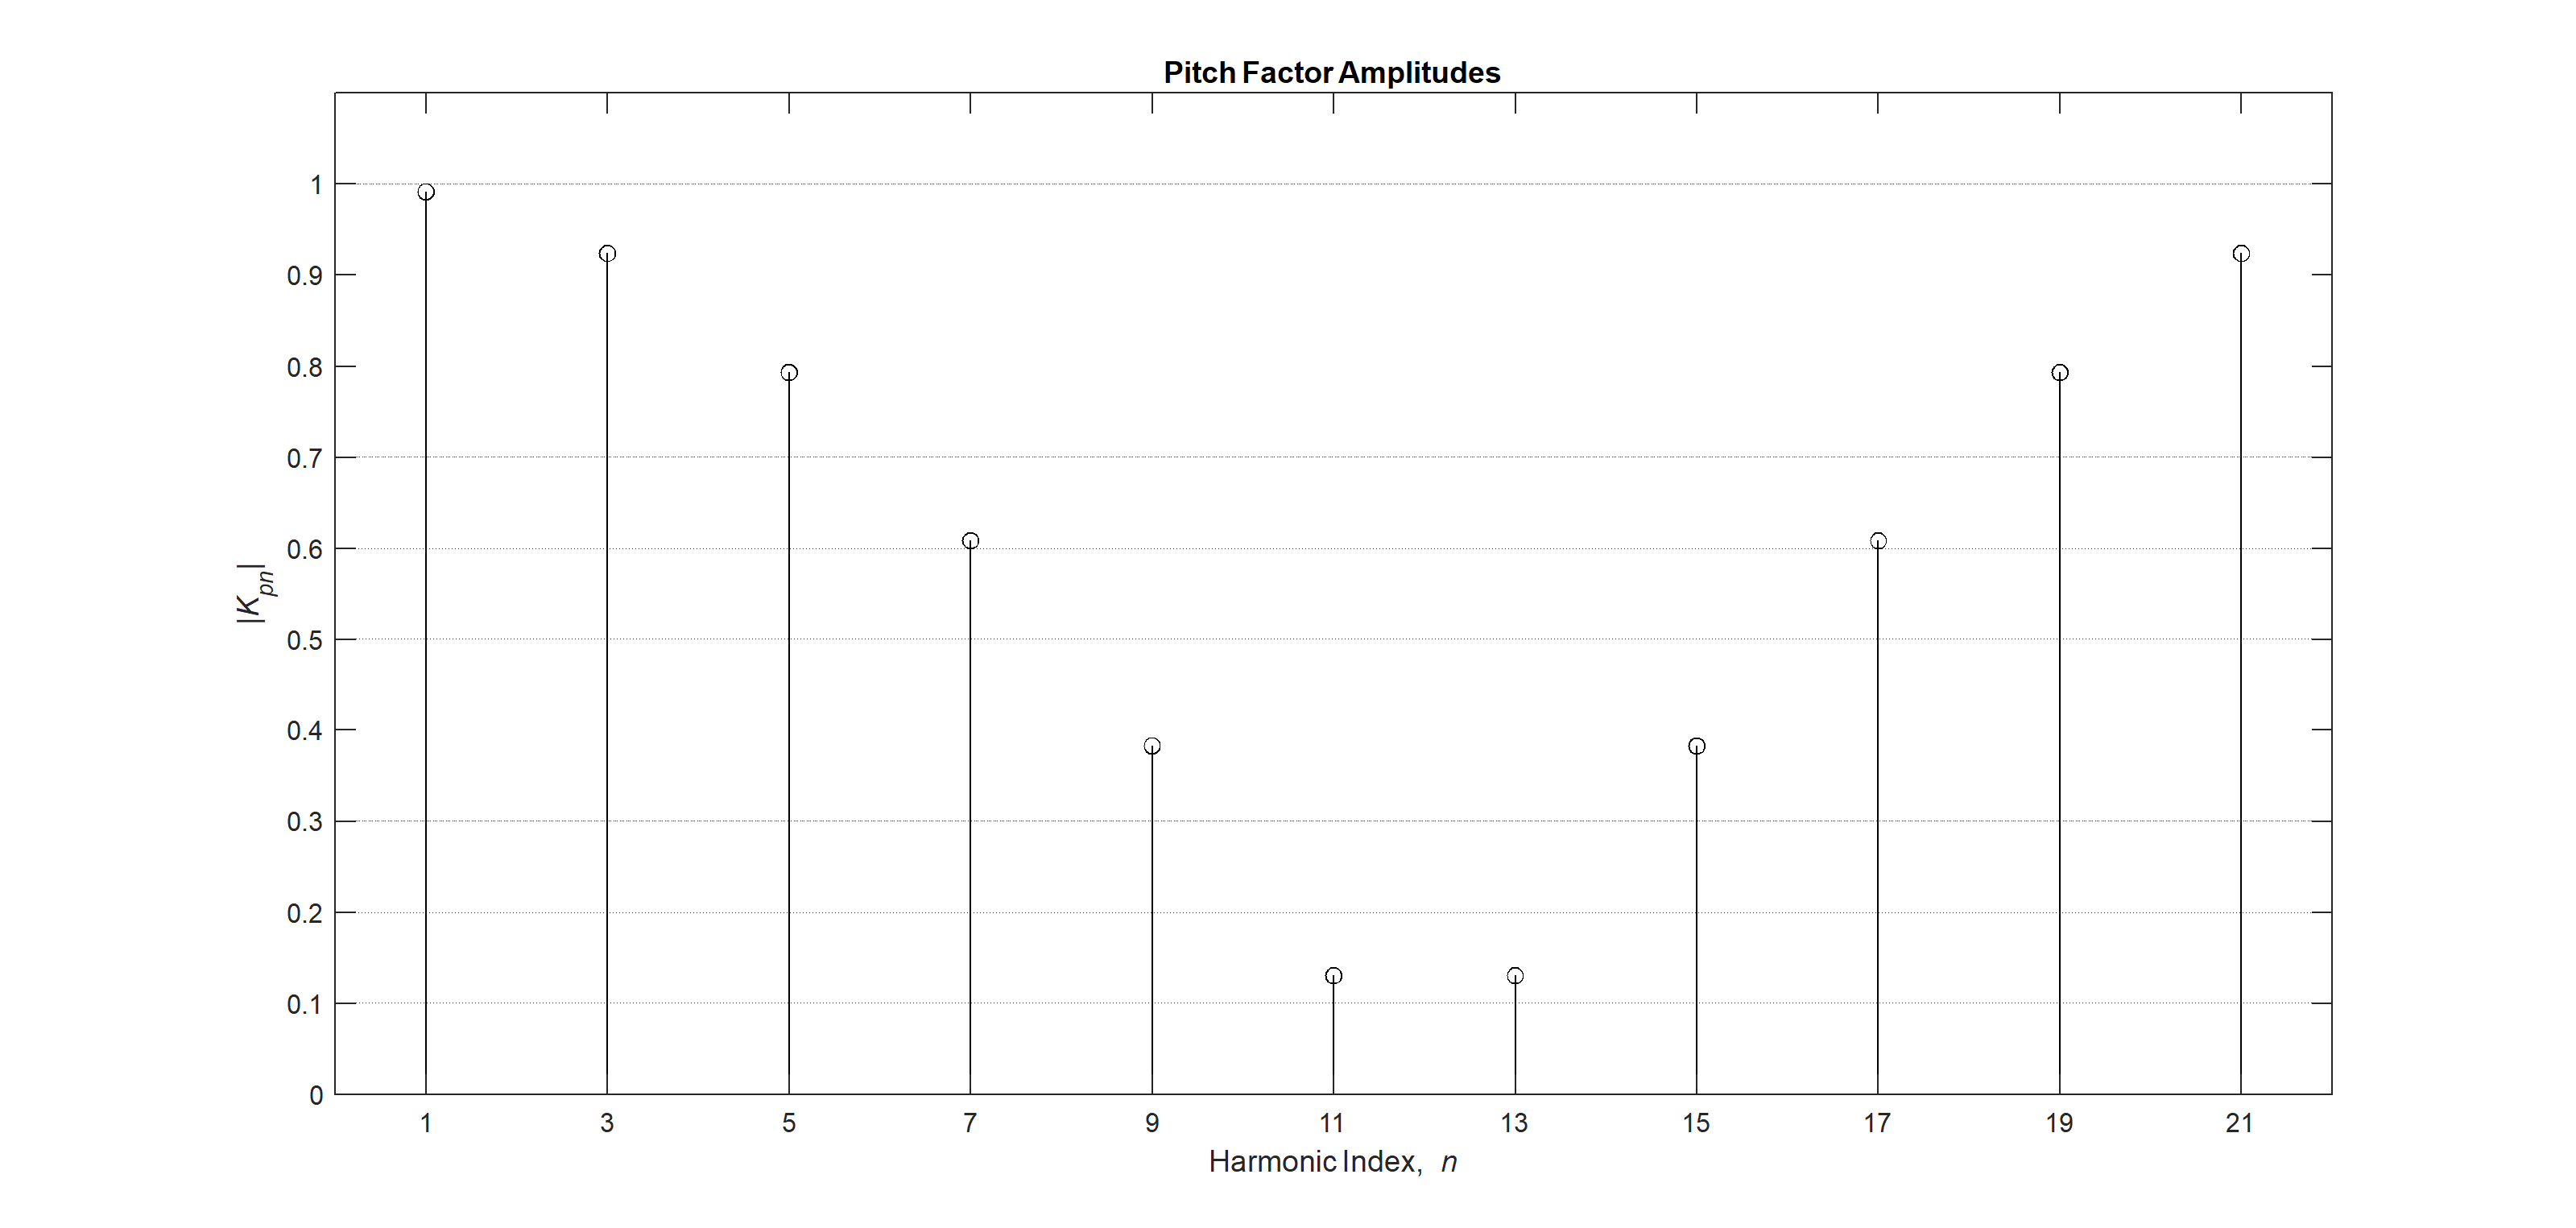
\includegraphics[width=\textwidth]{Q2_2422_pitchFactor.png}
        \caption{}
        \label{subfig:Q2_pitch_factor_2422}
    \end{subfigure}
    \begin{subfigure}[b]{1.00\textwidth}
        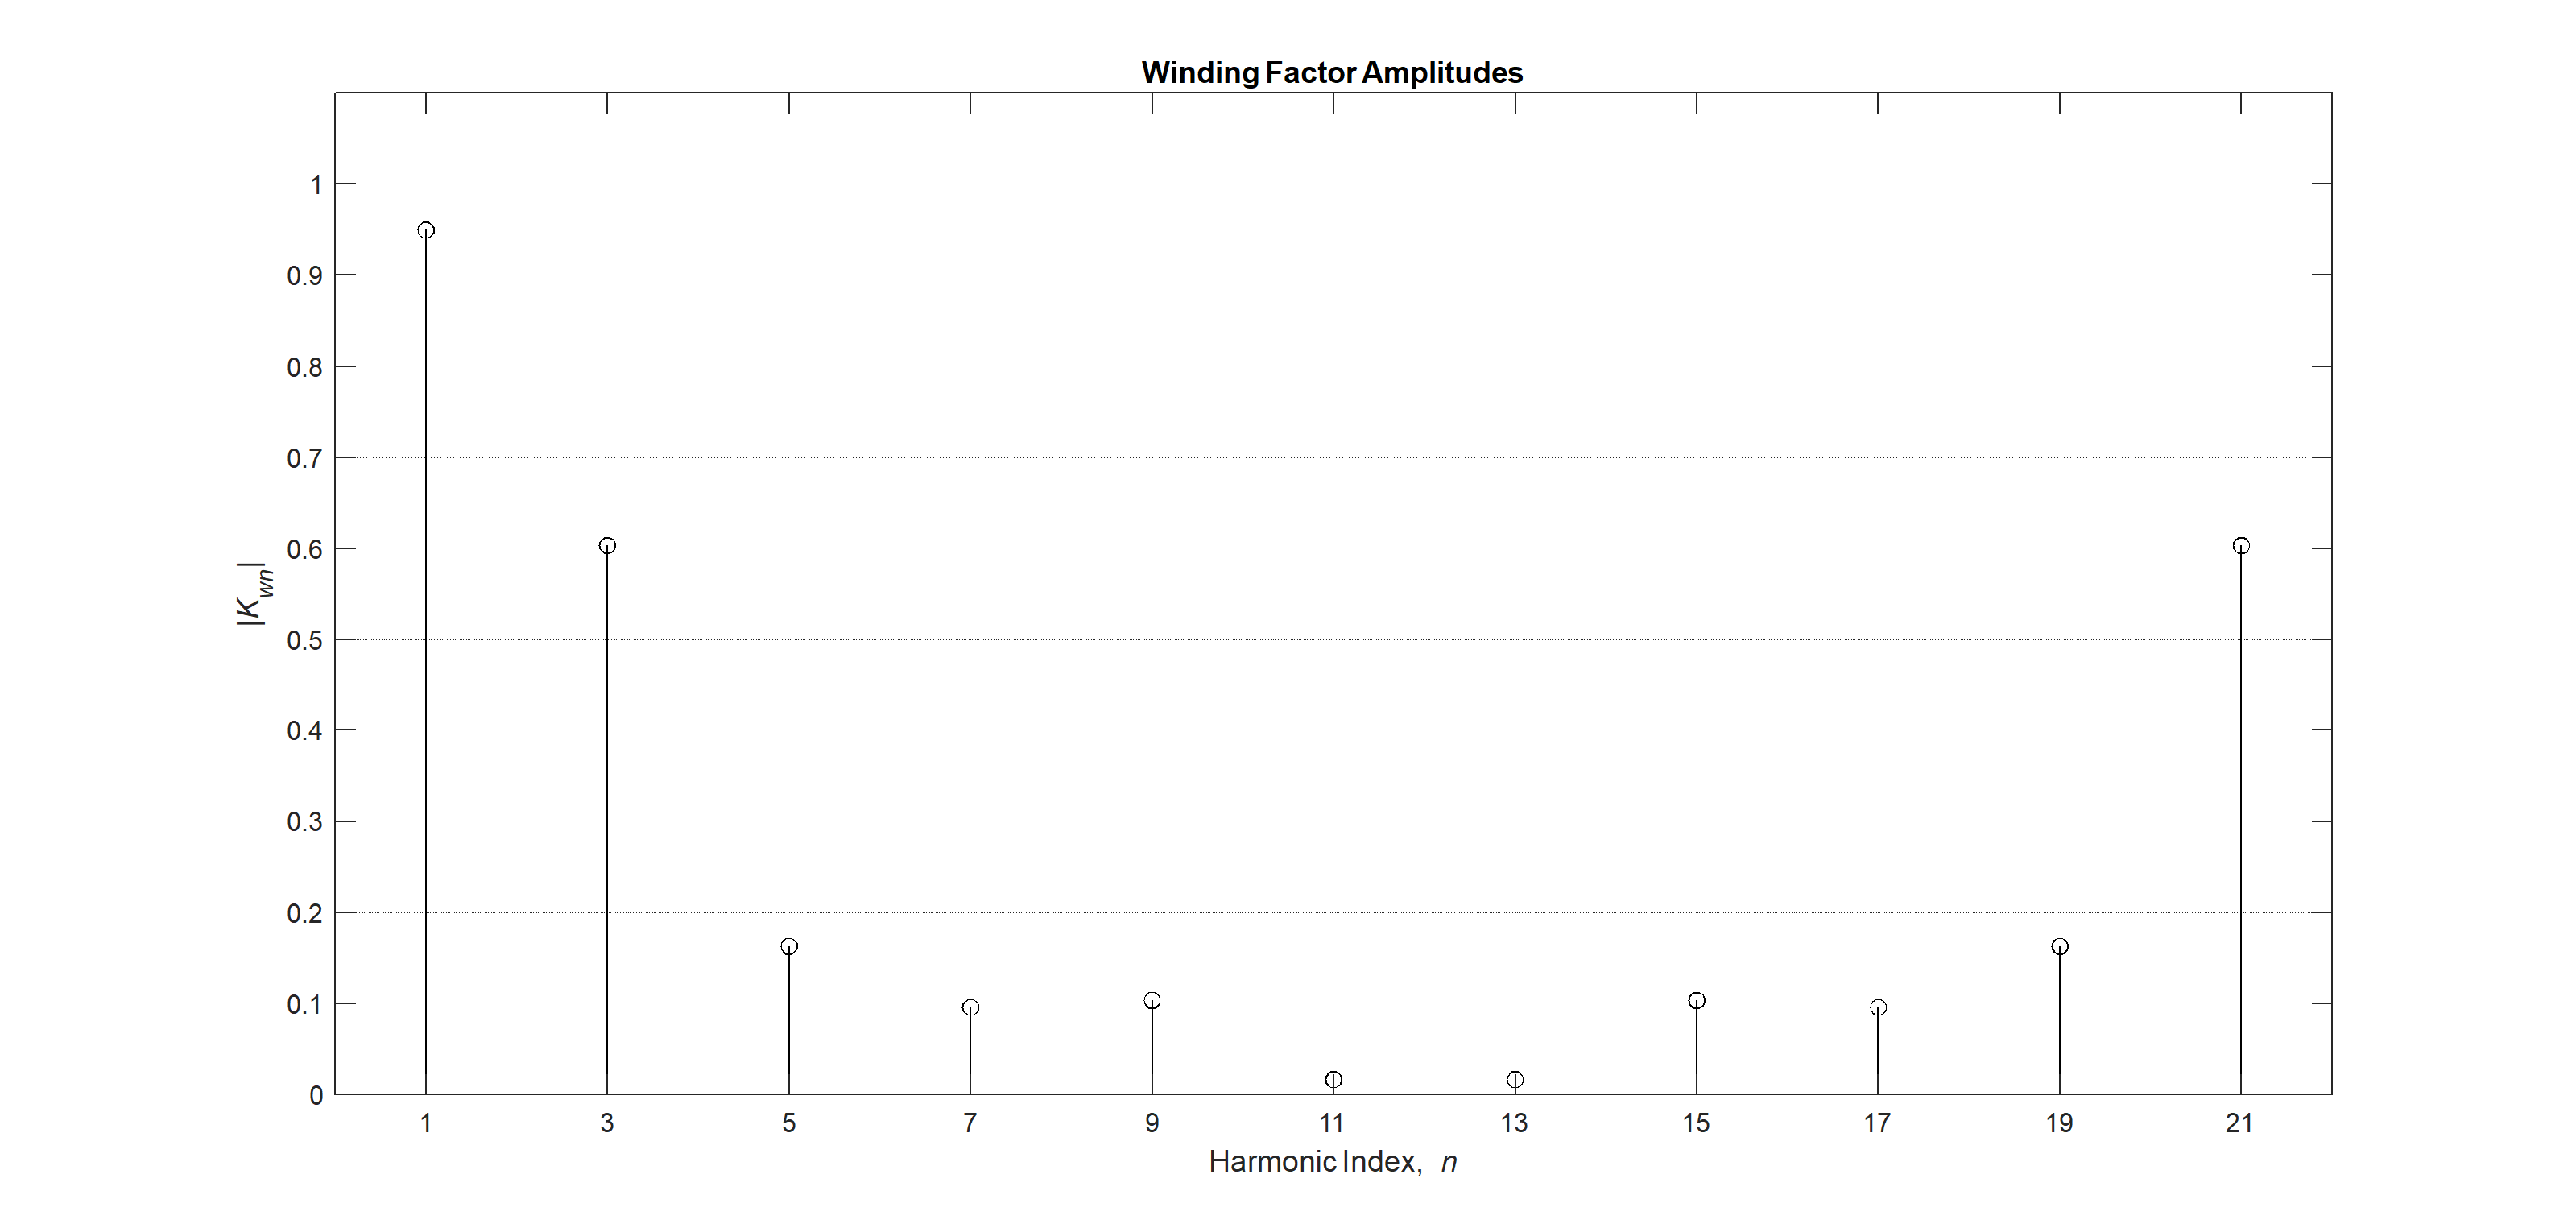
\includegraphics[width=\textwidth]{Q2_2422_windingFactor.png}
        \caption{}
        \label{subfig:Q2_wind_factor_2422}
    \end{subfigure}
    \caption{Distribution, Pitch and Winding Factor for $\frac{N_s}{2p}=24/22$}
    \label{fig:Q2_factors_2422}
\end{figure}

Again here, as can be seen in Figure \ref{tab:Q2_factors_2422}, the fundamental distribution factor calculated analytically with the Equation \ref{eq:distribution_factor_arithmetic} gives the same results with that calculated by the phasor diagram in \ref{subsubsec:phasor_d_2422}.

\subsection{Evaluation}

Fundamental component winding factor is very similar in these two designs, though higher for $\frac{N_s}{2p}=24/22$ than $\frac{N_s}{2p}=27/22$,  i.e $K_{w1} =0.9495$ for $\frac{N_s}{2p}=24/22$ and $K_{w1} =0.9153$ for $\frac{N_s}{2p}=27/22$, as can be seen in Table \ref{tab:Q2_factors_2722}, \ref{tab:Q2_factors_2422}. Fundamental component of pitch factor for $\frac{N_s}{2p}=24/22$ is $K_{p1} =0.9914$, while for $\frac{N_s}{2p}=27/22$ it is $K_{p1} =0.9580$. The fundamental component of the distribution factors are very similar, i.e. $K_{d1} =0.9577$ for $\frac{N_s}{2p}=24/22$ and $K_{d1} =0.9555$ for $\frac{N_s}{2p}=27/22$. Therefore, pitch factors are the main contributers to this result.

The 3\textsuperscript{rd} and the 5\textsuperscript{th} harmonic component of winding factor diminish faster for the design with $\frac{N_s}{2p}=27/22$ than $\frac{N_s}{2p}=24/22$, as can be seen in Figure \ref{subfig:Q2_wind_factor_2722}, \ref{subfig:Q2_wind_factor_2422} and Table \ref{tab:Q2_factors_2722}, \ref{tab:Q2_factors_2422}. In case of $\frac{N_s}{2p}=24/22$, the winding factor decreases from $K_{w1} =0.9495$ at fundamental component, to $K_{w3} =0.6036$ at 3\textsuperscript{rd} harmonic, and then to  $K_{w5} =0.1629$ at 5\textsuperscript{th} harmonic, while in case of $\frac{N_s}{2p}=27/22$, the winding factor decreases from $K_{w1} =0.9153$ at fundamental component, to $K_{w3} =0.4113$ at 3\textsuperscript{rd} harmonic, and then to  $K_{w5} =0.0225$ at 5\textsuperscript{th} harmonic. This is again the result of pitch factor values at 3\textsuperscript{rd} and  5\textsuperscript{th} harmonic component. The distribution factor decreases in similar fashion for both $\frac{N_s}{2p}=27/22$ and $\frac{N_s}{2p}=24/22$. However, the pitch factor plummets at 5\textsuperscript{th} harmonic component for $\frac{N_s}{2p}=27/22$, while it takes almost 11\textsuperscript{th} harmonic for $\frac{N_s}{2p}=24/22$ pitch factor to decrease to that levels.

The fundamental component distribution factors for both designs are similar. This was expected after constructing the single phase phasor diagram for $\frac{N_s}{2p}=27/22$ in Figure \ref{fig:phasor_d_2722}. The phasor diagram for $\frac{N_s}{2p}=27/22$ contains 9 phasors, one more phasor than that for $\frac{N_s}{2p}=24/22$, which has 8 phasors. The phasor diagram for $\frac{N_s}{2p}=27/22$ has one extra phasor that is in the same direction as phase A, which increases the distribution factor. However, the phasors spread further away from phase A in $\frac{N_s}{2p}=27/22$, as can be seen in Figure \ref{fig:sos_2722_wSectors}, \ref{fig:sos_2422_wSectors}. This, in turn, decreases the distribution factor. Overall, the two adjustments happen on the phasors as the design changes from $\frac{N_s}{2p}=27/22$ to $\frac{N_s}{2p}=24/22$ have opposite effects on distribution factor, working against each other. Thus the overall effect on distribution factor is small.


\section{2-D FEA Modelling: 27-slot/22-pole EM}

The machine with $\frac{N_s}{2p}=27/22$ winding design is modelled in 2 dimensions. \textit{ANSYS RMxprt} is used to model the machine. The parameters presented at \textit{Chapter 10: Examples} of Hanselman's book are adopted as the design parameters \cite{hanselman}. Overall, the machine simulation results present an efficiency of $\%71.4257$ at full-load operation. This efficiency rating is less than the general efficiency ratings achieved with permanent magnet synchronous machines; therefore, the model needs further optimization.

\begin{table}[h!]
\centering
	\begin{tabular}{|| c | c || c | c ||} 
		\hline\hline
		Electrical Steel & M19 M4G & Rated Output Power & 20 kW \\ [0.5ex] 
		\hline
		Stacking Factor & 0.95 & Rated Voltage & 138 \\ 
		\hline
		Conductors per Slot & 52 & Rated Speed & 1000 rpm \\
		\hline
		Winding Factor & 0.9495 & Operating Temperature & 50\degree \\
		Magnet Type & Arnold Magnetics N45 & \degree \\
		\hline\hline
	\end{tabular}
	\caption{Machine Parameters}
	\label{tab:Q3_machineParameters}
\end{table}



\subsection{2-D drawing and winding diagram}

The 2 dimensional model as it is depicted in the simulation environment can be seen in Figure \ref{fig:Q3_2D}, below.
\begin{figure}[h!]
    \centering
	\begin{center}
		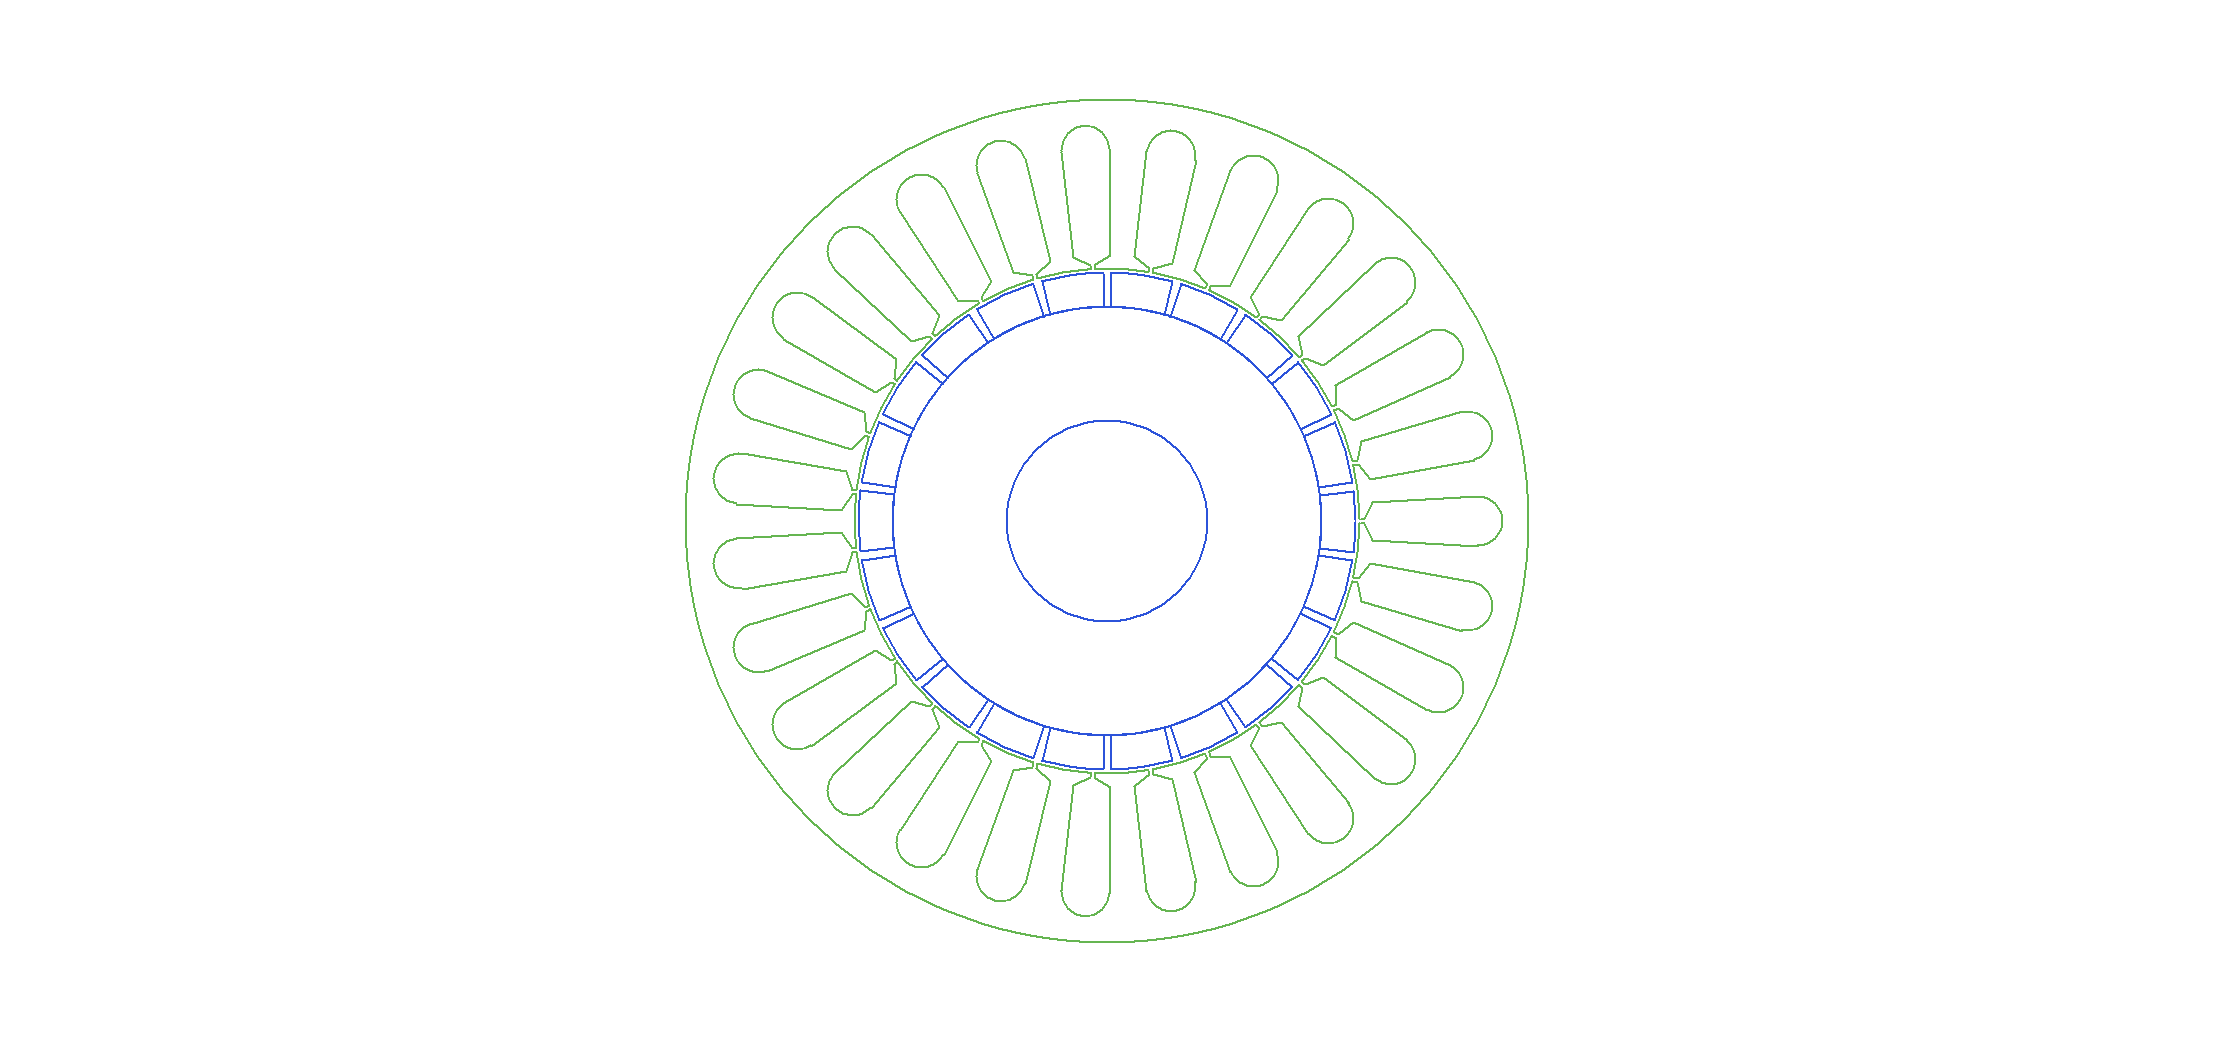
\includegraphics[width=1.0\textwidth]{Q3_2D.png}
	\end{center}
	\caption{General 2-D Drawing}
	\label{fig:Q3_2D}
\end{figure}

\begin{figure}[h!]
    \centering
	\begin{center}
		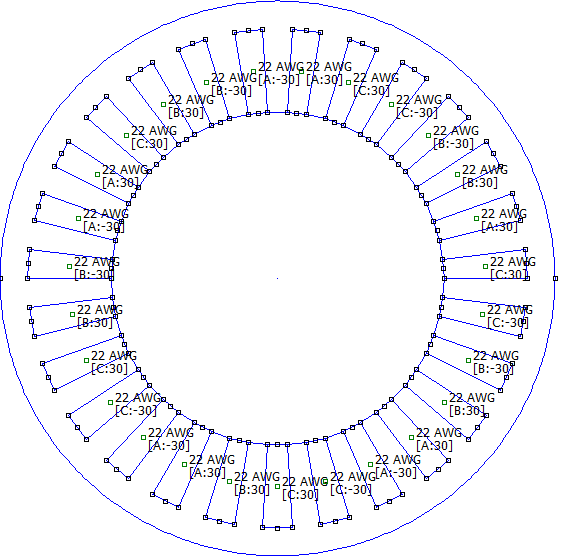
\includegraphics[width=0.6\textwidth]{Q3_2D_FEMM.png}
	\end{center}
	\caption{Stator 2-D Drawing (FEMM)}
	\label{fig:Q3_2D_FEMM}
\end{figure}

The winding diagram as it is depicted in the simulation environment can be seen in Figure \ref{fig:Q3_windingDiagram}, below. It is apparent that each coil spans 1 slot.

\begin{figure}[h!]
    \centering
	\begin{center}
		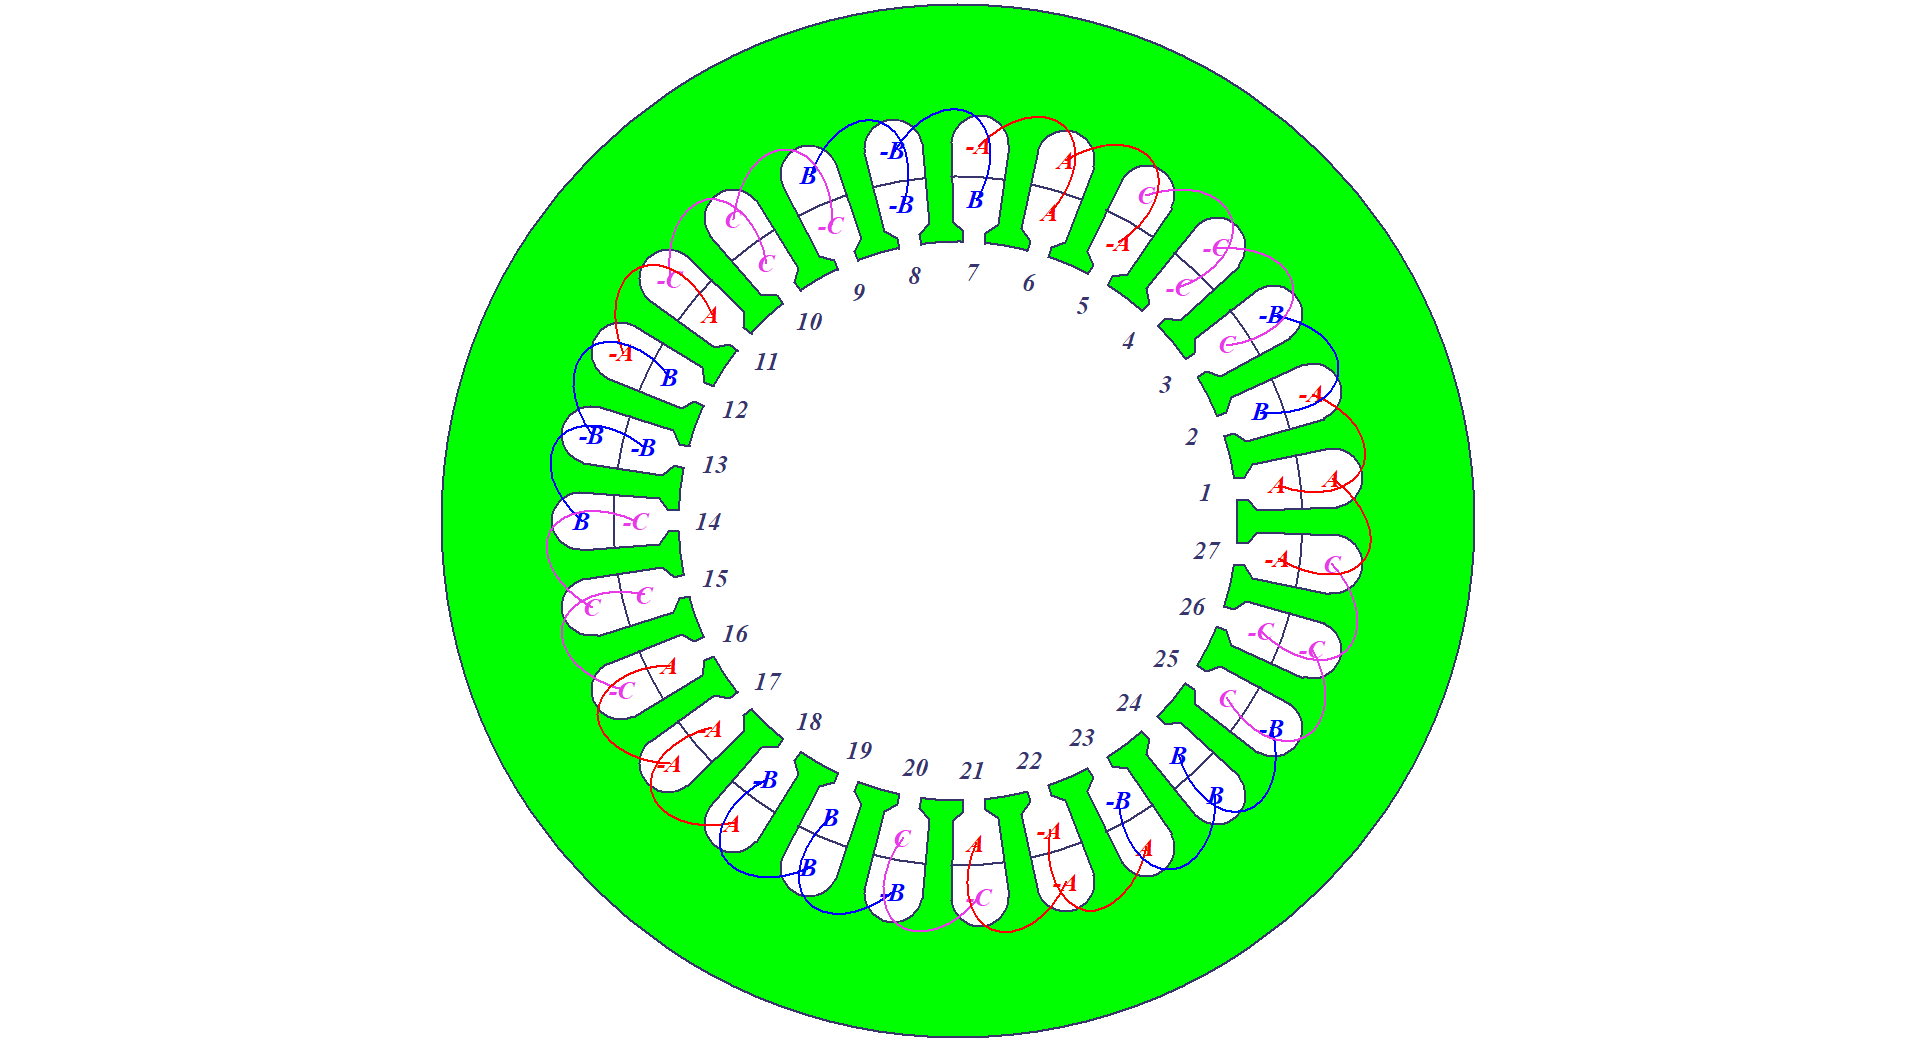
\includegraphics[width=1.0\textwidth]{Q3_winding_diagram.png}
	\end{center}
	\caption{Winding Diagram}
	\label{fig:Q3_windingDiagram}
\end{figure}

\subsection{Airgap flux density distribution}

The airgap flux density is plotted by the \textit{RMxprt} simulation and can be seen in Figure \ref{fig:Q3_airgapFluxDensity}, below. It can be seen that the airgap flux density varies between $-0.82T$ and $0.82T$.

\begin{figure}[h!]
    \centering
	\begin{center}
		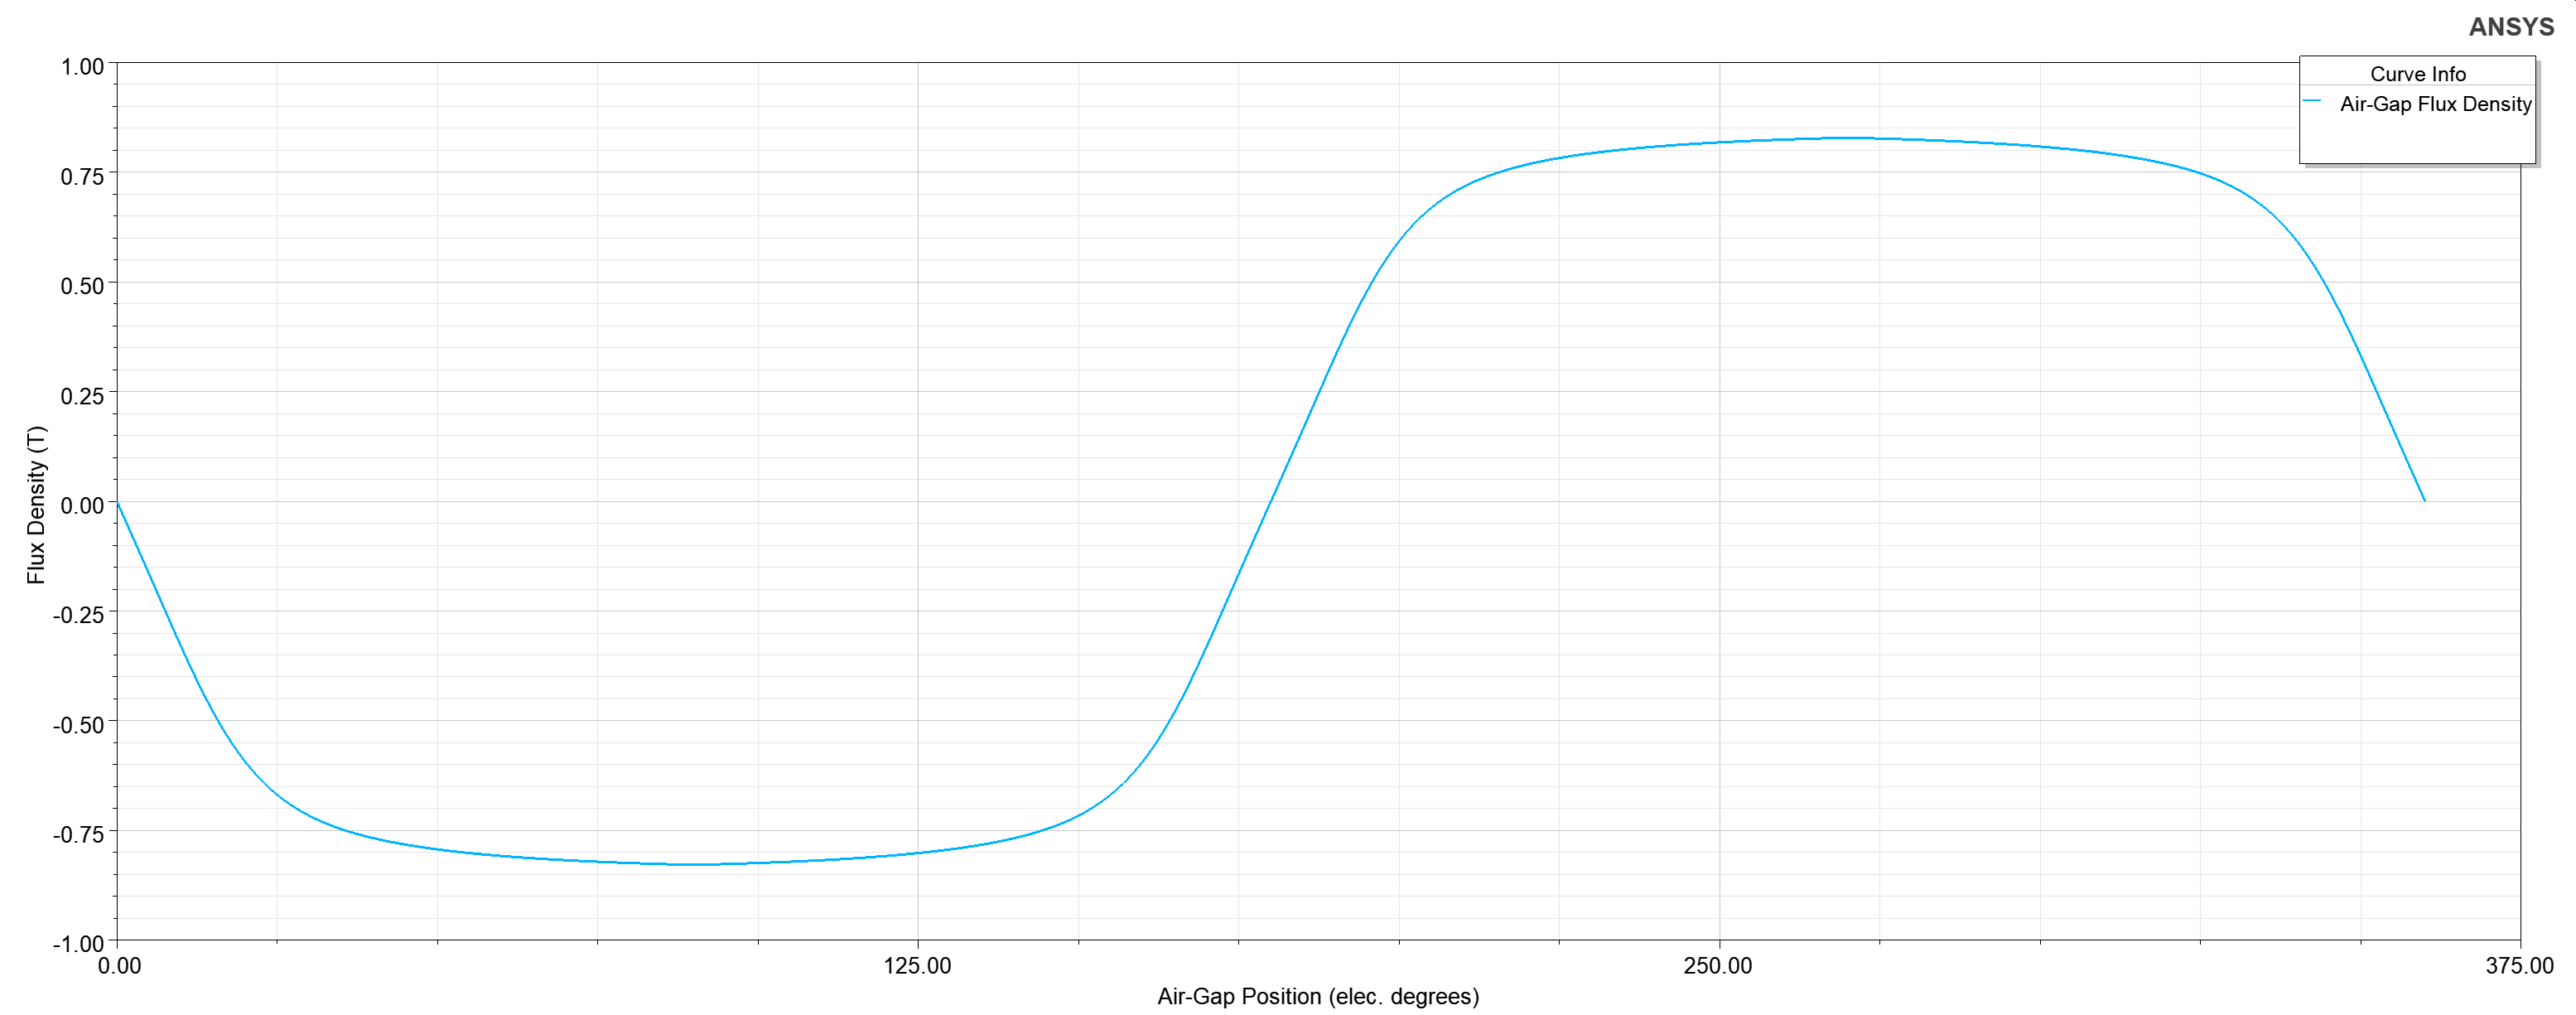
\includegraphics[width=0.8\textwidth]{Q3_airgapFluxDensity.png}
	\end{center}
	\caption{Airgap Flux Density}
	\label{fig:Q3_airgapFluxDensity}
\end{figure}

\subsection{Induced voltage waveforms (for phase and line-to-line) at rated speed}


The induced voltage waveforms (for phase and line-to-line) at rated speed are plotted by the \textit{RMxprt} simulation and can be seen in Figure \ref{fig:Q3_inducedVoltageWaveforms}, below.
\begin{figure}[h!]
    \centering
	\begin{center}
		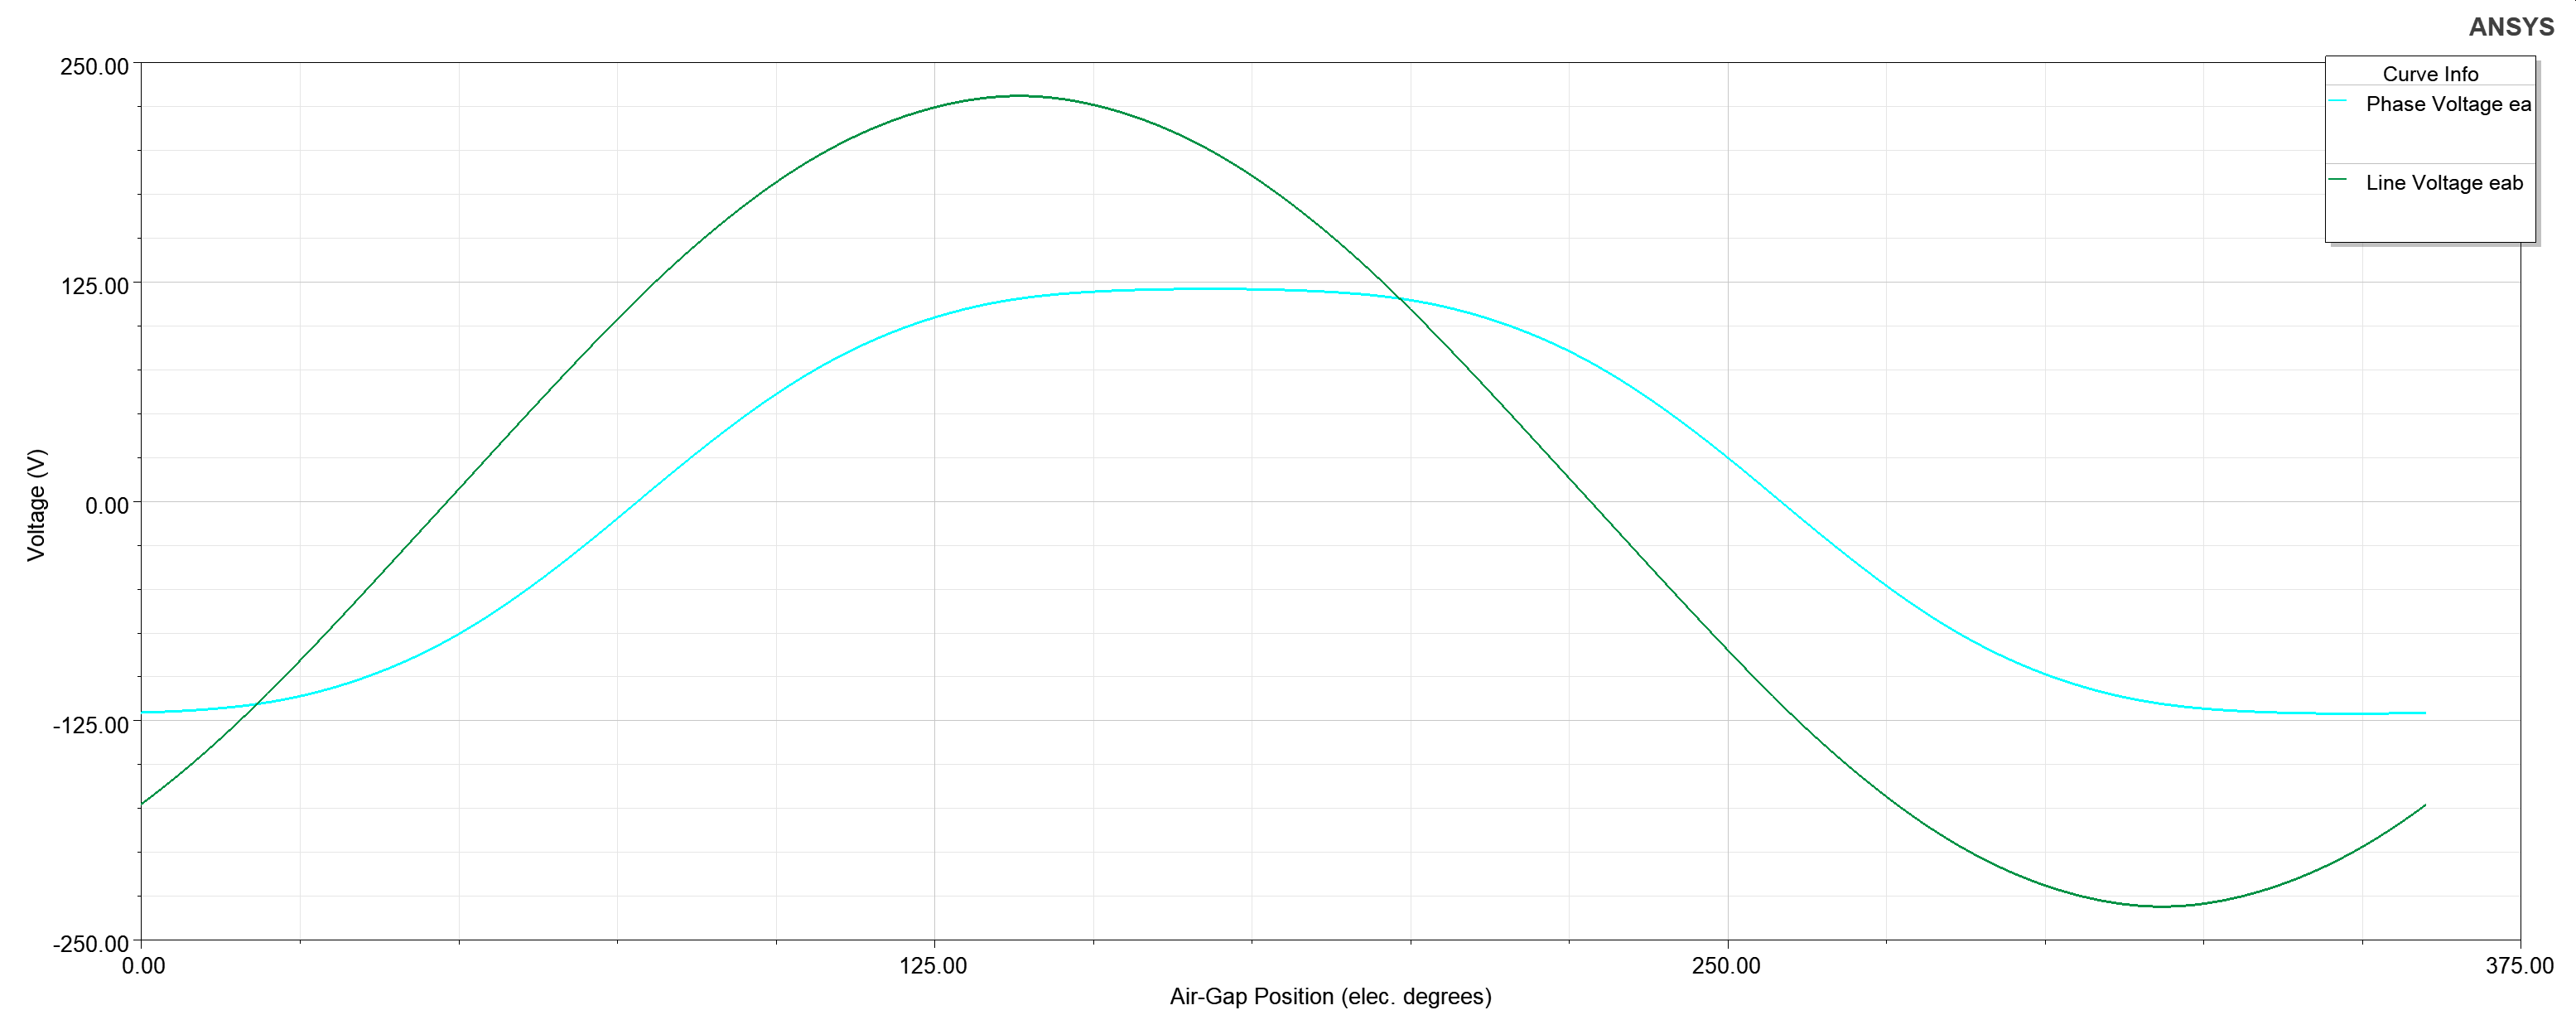
\includegraphics[width=1.0\textwidth]{Q3_inducedVoltageWaveforms}
	\end{center}
	\caption{Induced Voltage Waveforms (for phase and line-to-line) at rated speed)}
	\label{fig:Q3_inducedVoltageWaveforms}
\end{figure}


\subsection{Cogging torque}

The cogging torque is plotted by the \textit{RMxprt} simulation and can be seen in Figure \ref{fig:Q3_coggingTorque}, below. As can be seen in Figure \ref{subfig:Q2_pitch_factor_2422}, cogging torque varies between $0.013 Nm$ and $-0.013 Nm$. The rated torque at full-load operation is obtained as $15.6622 Nm$ from the software. Therefore, the cogging torque is $\%0.08$ of the rated torque.


\begin{figure}[h!]
    \centering
    \begin{subfigure}[b]{1.00\textwidth}
        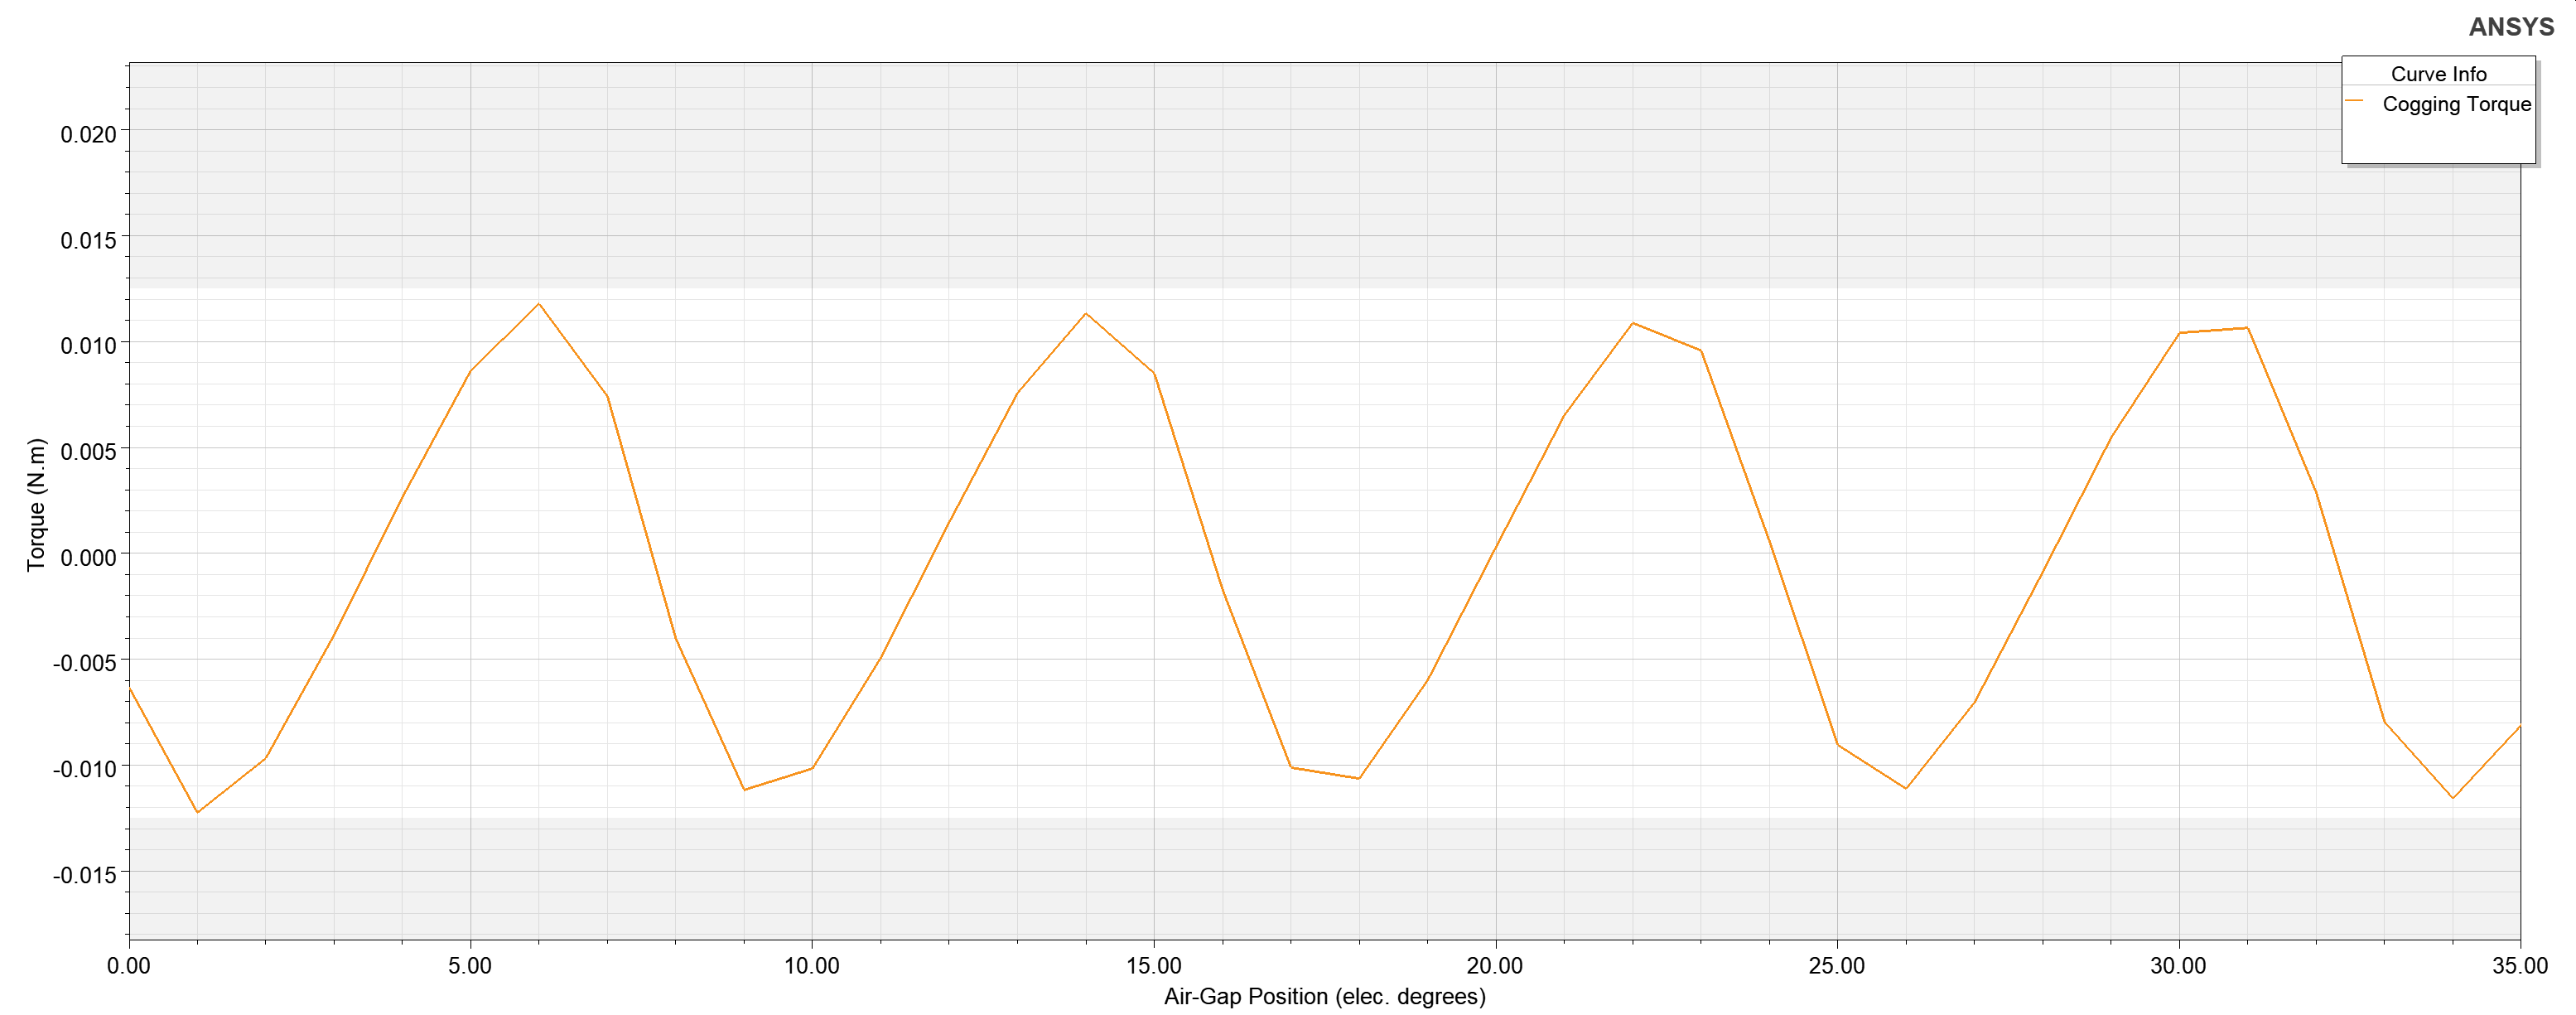
\includegraphics[width=\textwidth]{Q3_coggingTorque_0to35.png}
        \caption{}
        \label{subfig:Q2_dist_factor_2422}
    \end{subfigure}
    \begin{subfigure}[b]{1.00\textwidth}
        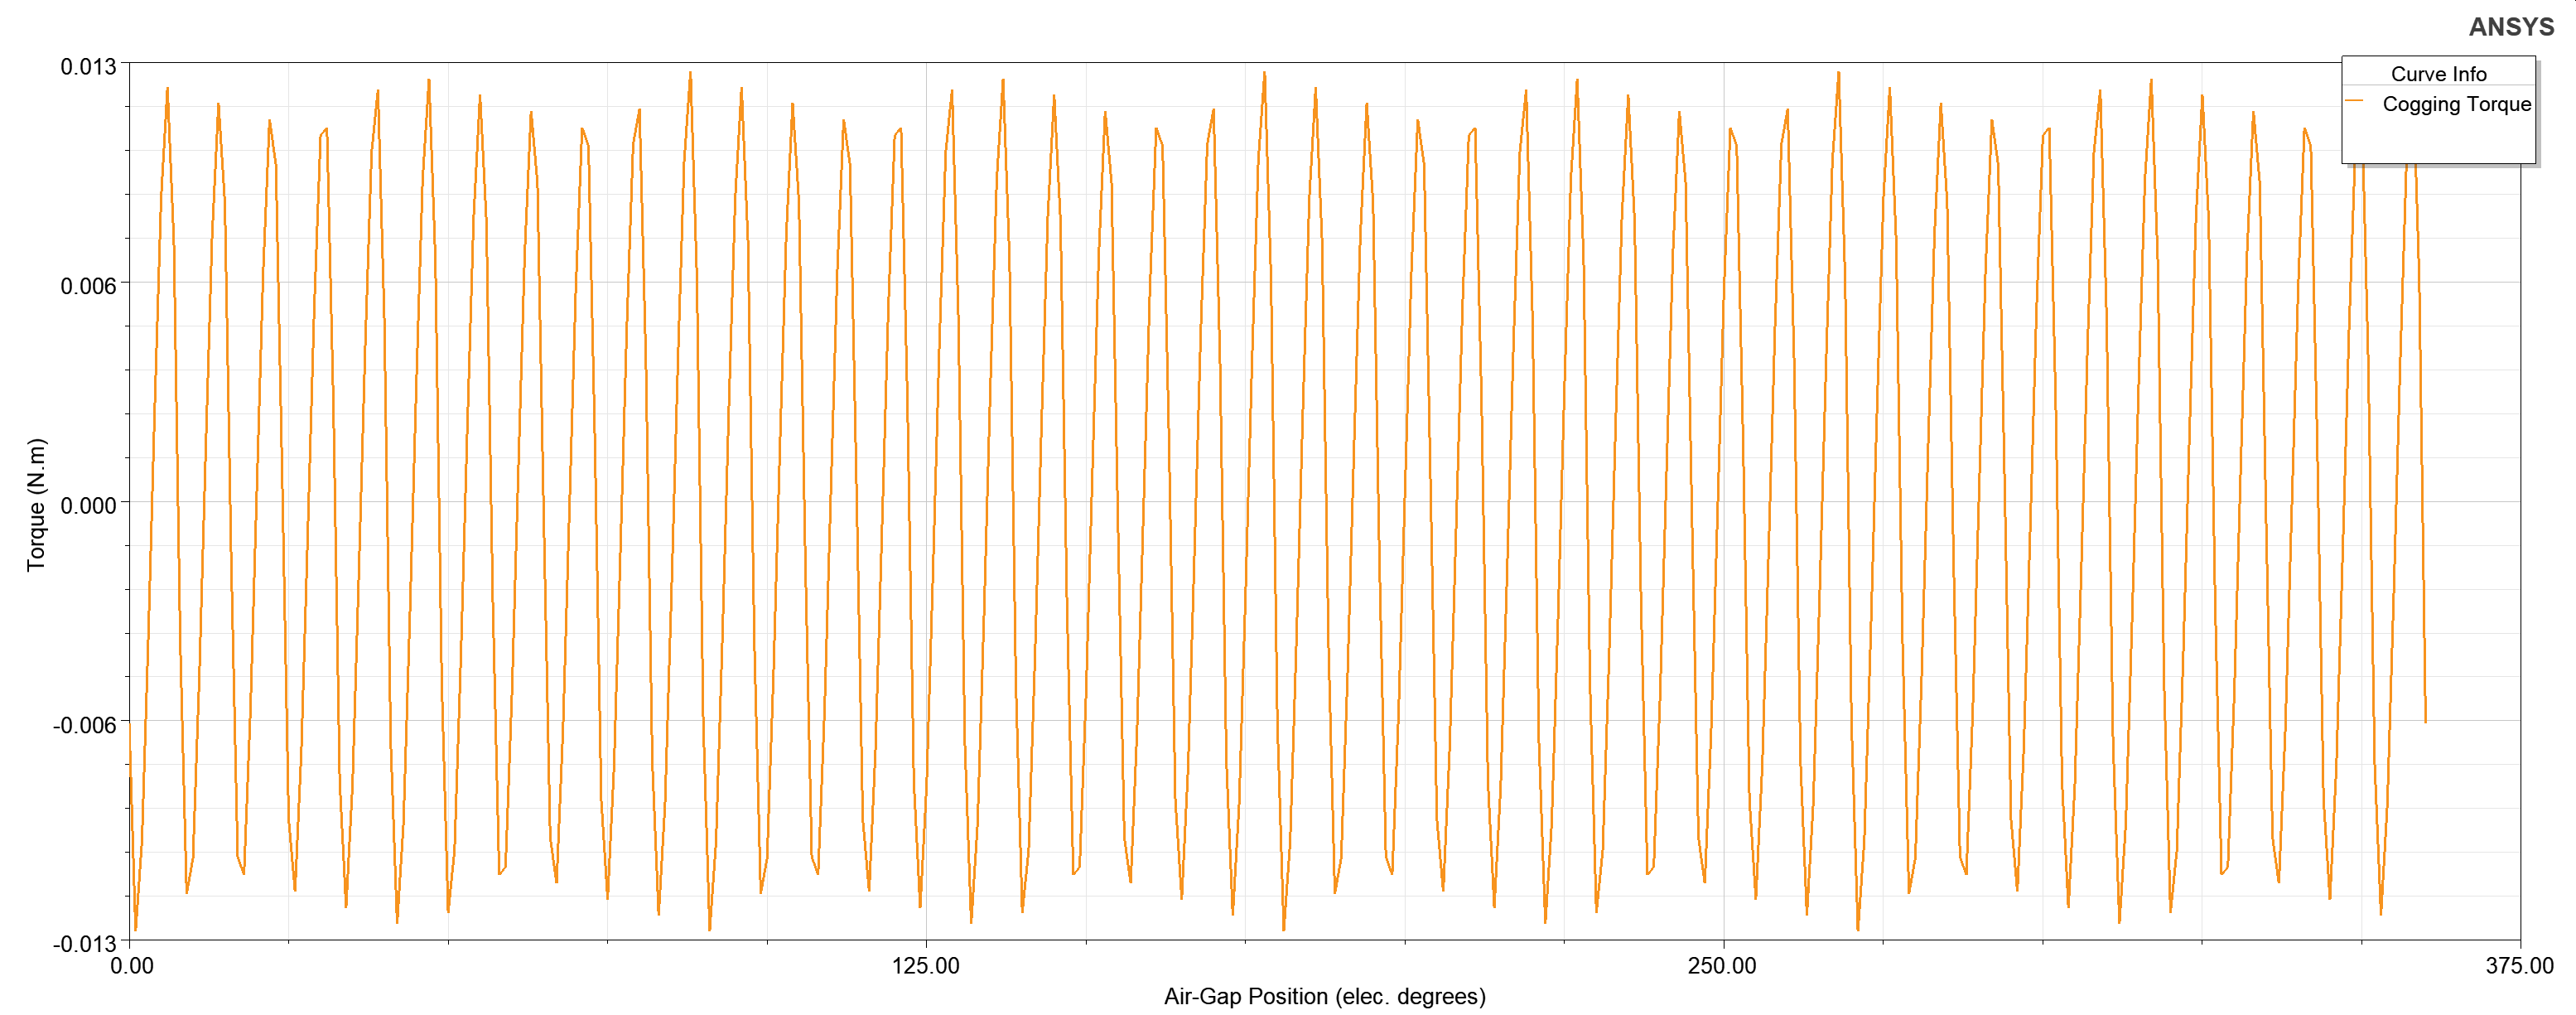
\includegraphics[width=\textwidth]{Q3_coggingTorque_0to360.png}
        \caption{}
        \label{subfig:Q2_pitch_factor_2422}
    \end{subfigure}
    \caption{Cogging Torque in two Teeth}
    \label{fig:Q3_coggingTorque}
\end{figure}

\newpage

\bibliography{bibliography} 
\bibliographystyle{plain}

\end{document}